\documentclass[technote, transmag, onecolumn, 9pt]{IEEEtran}

\makeatletter
\long\def\@makecaption#1#2{\ifx\@captype\@IEEEtablestring%
\footnotesize\begin{center}{\normalfont\footnotesize #1}\\
{\normalfont\footnotesize\scshape #2}\end{center}%
\@IEEEtablecaptionsepspace
\else
\@IEEEfigurecaptionsepspace
\setbox\@tempboxa\hbox{\normalfont\footnotesize {#1.}~~ #2}%
\ifdim \wd\@tempboxa >\hsize%
\setbox\@tempboxa\hbox{\normalfont\footnotesize {#1.}~~ }%
\parbox[t]{\hsize}{\normalfont\footnotesize \noindent\unhbox\@tempboxa#2}%
\else
\hbox to\hsize{\normalfont\footnotesize\hfil\box\@tempboxa\hfil}\fi\fi}
\makeatother

\usepackage{graphicx}

\usepackage{csquotes}

\usepackage{listings}

% \usepackage{caption}

\ifCLASSOPTIONcompsoc
\usepackage[caption=false,font=normalsize,labelfont=sf,textfont=sf]{subfig}
\else
\usepackage[caption=false,font=footnotesize]{subfig}
\fi

\usepackage[export]{adjustbox}

\usepackage{array}
\newcolumntype{L}[1]{>{\raggedright\let\newline\\\arraybackslash\hspace{0pt}}p{#1}}
\newcolumntype{C}[1]{>{\centering\let\newline\\\arraybackslash\hspace{0pt}}p{#1}}
\newcolumntype{R}[1]{>{\raggedleft\let\newline\\\arraybackslash\hspace{0pt}}p{#1}}

\title{2021 FALL COEN6311 Assignment 1 Report}

% \author{
%     \IEEEauthorblockN{Jun Huang}
%     \IEEEauthorblockA{40168167\\Email: youyinnn@foxmail.com}
% }

\author{Jun Huang\\40168167\\Email: youyinnn@foxmail.com}

\begin{document}

\maketitle

\section{Deliverable Specification}

\subsection*{\textbf{D1-User Stories and Use Cases}}

According to the project description, the user stories of the system can be listed as follow:

\begin{enumerate}
	\item The user wants to track the GPS data of the bike which represent on a digital map,
	      so he can know the real-time location of it.
	\item The user wants to know the speed of the bike, so he can know if he can catch the moving stolen bike.

	\item The user wants to set a \textquote{Parked} state to the bike,
	      so the chip(micro-controller) would treat the any swing as a threat of stealing.

	\item The user wants to set the \textquote{Unparked} state to the bike,
	      so the chip would not treat the swing perform by the user as a threat of stealing.

	\item The user wants to know if the bike was swinging or not,
	      so he can know if someone was attempting to move his bike or to break his lock.

	\item The user wants to get the real-time notifications which described above,
	      so he can know the state of the bike immediately.
\end{enumerate}

The use cases diagram is shown in Fig. \ref{fig:use-cases}.

\begin{figure}[!hb]
	\centering
	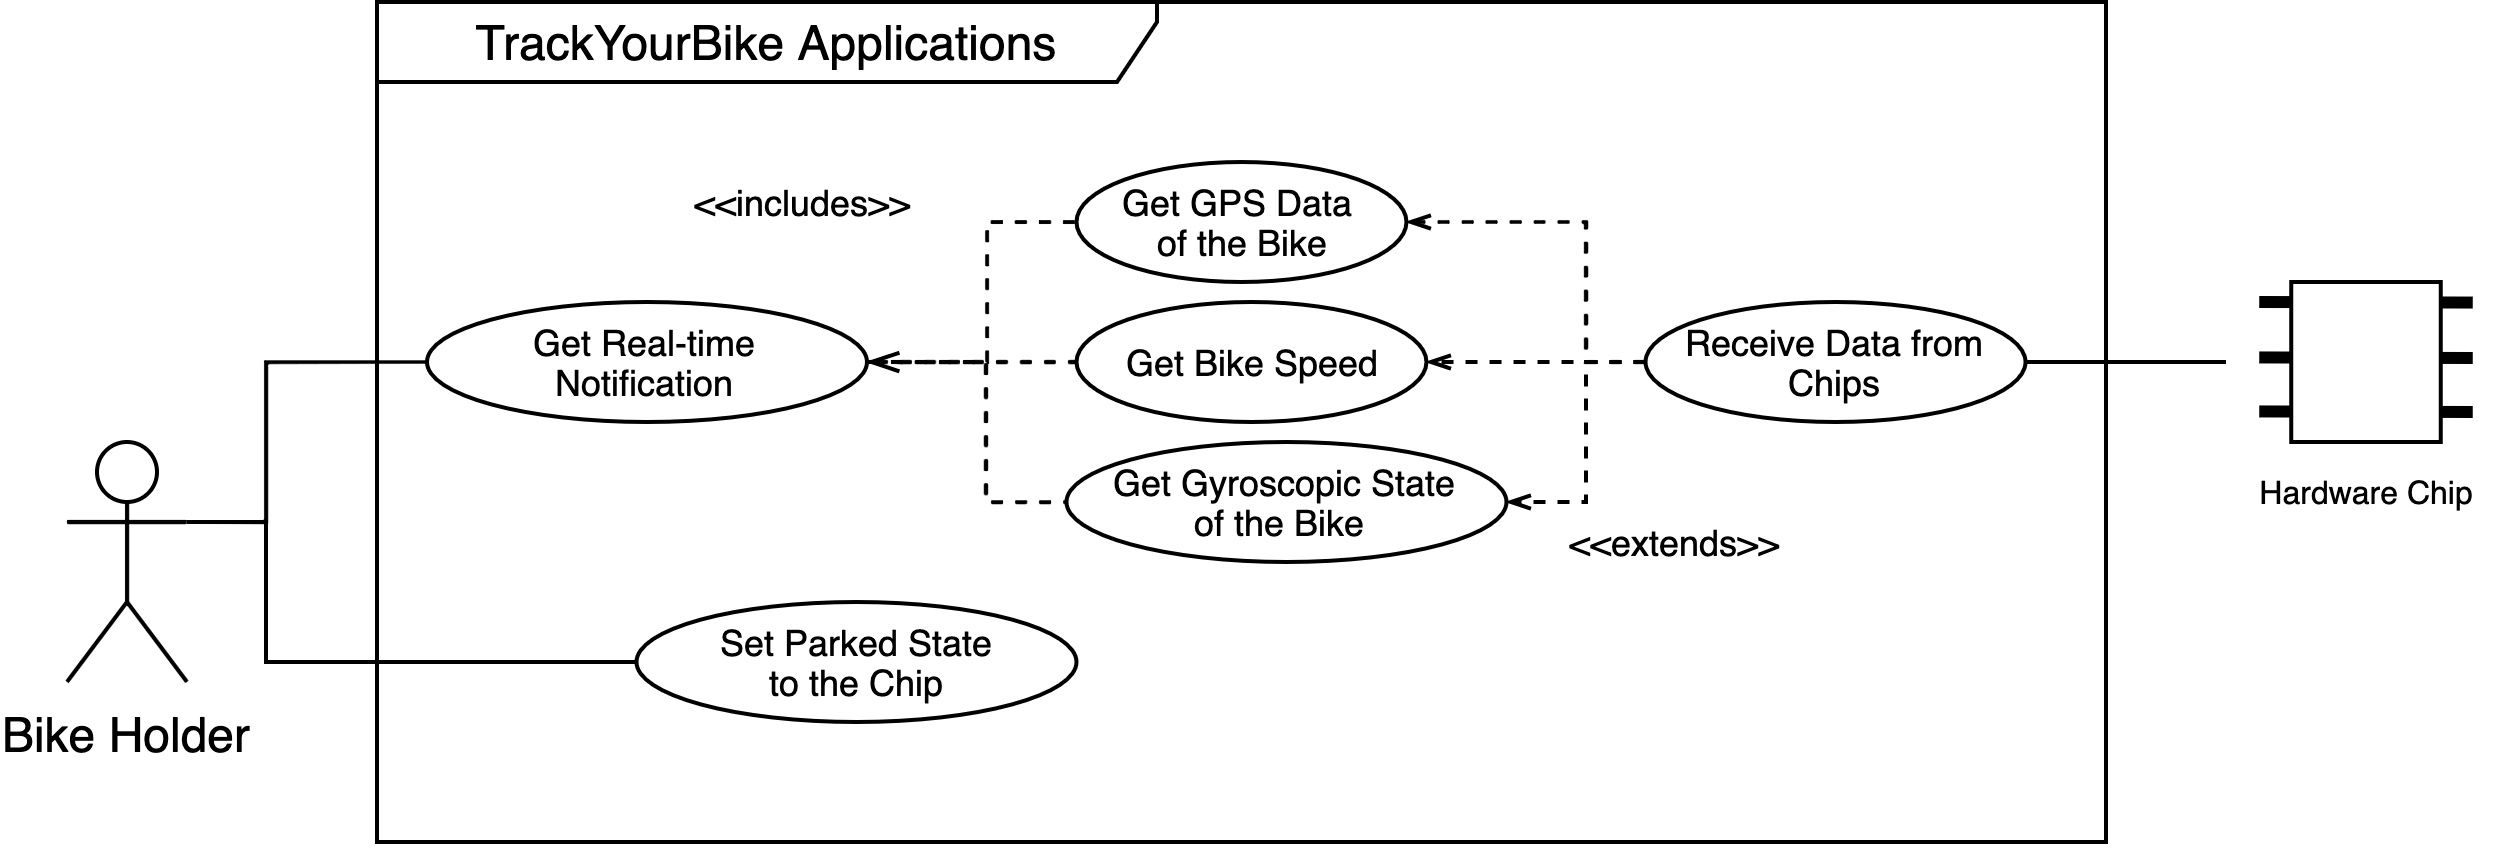
\includegraphics[width=0.8\textwidth]{./img/f1-use-cases.png}
	\caption{System Use Cases}
	\label{fig:use-cases}
\end{figure}

\subsection*{\textbf{D2-System Requirement Specification}}

Based on the user scenairo and the use cases,
the software shall have the following software requirement specifications and their sub-requirements.

To fulfill the described software product, the overall product should contains at least 3 software systems:

\begin{itemize}
	\item \textit{Software on the Tracker Chip}: which will be installed in the hardware chip to perform tracking features
	      and send sensor data to the remote server.
	\item \textit{Cloud Server System}: which will be deployed on the cloud server and receive data from users' chips
	      then forwarding those data to users' applications.
	\item \textit{Client Application}: which will be installed on users' mobile devices
	      then receive and display the data or notification from the server,
	      and also will send instructions to the corresponding chips.
\end{itemize}

This report will focus on the \textit{Software on the Tracker Chip}
but also present part of the \textit{Cloud Server System} which is just for supplementary notes.
The \textit{Client Application} will not be presented.
Notice the SRS of the cloud system will be marked as \textit{Server-SRS} for distinction.

More information of the system context architecture is shown in Fig. \ref{fig:sys-context}.

\begin{figure}[!ht]
	\centering
	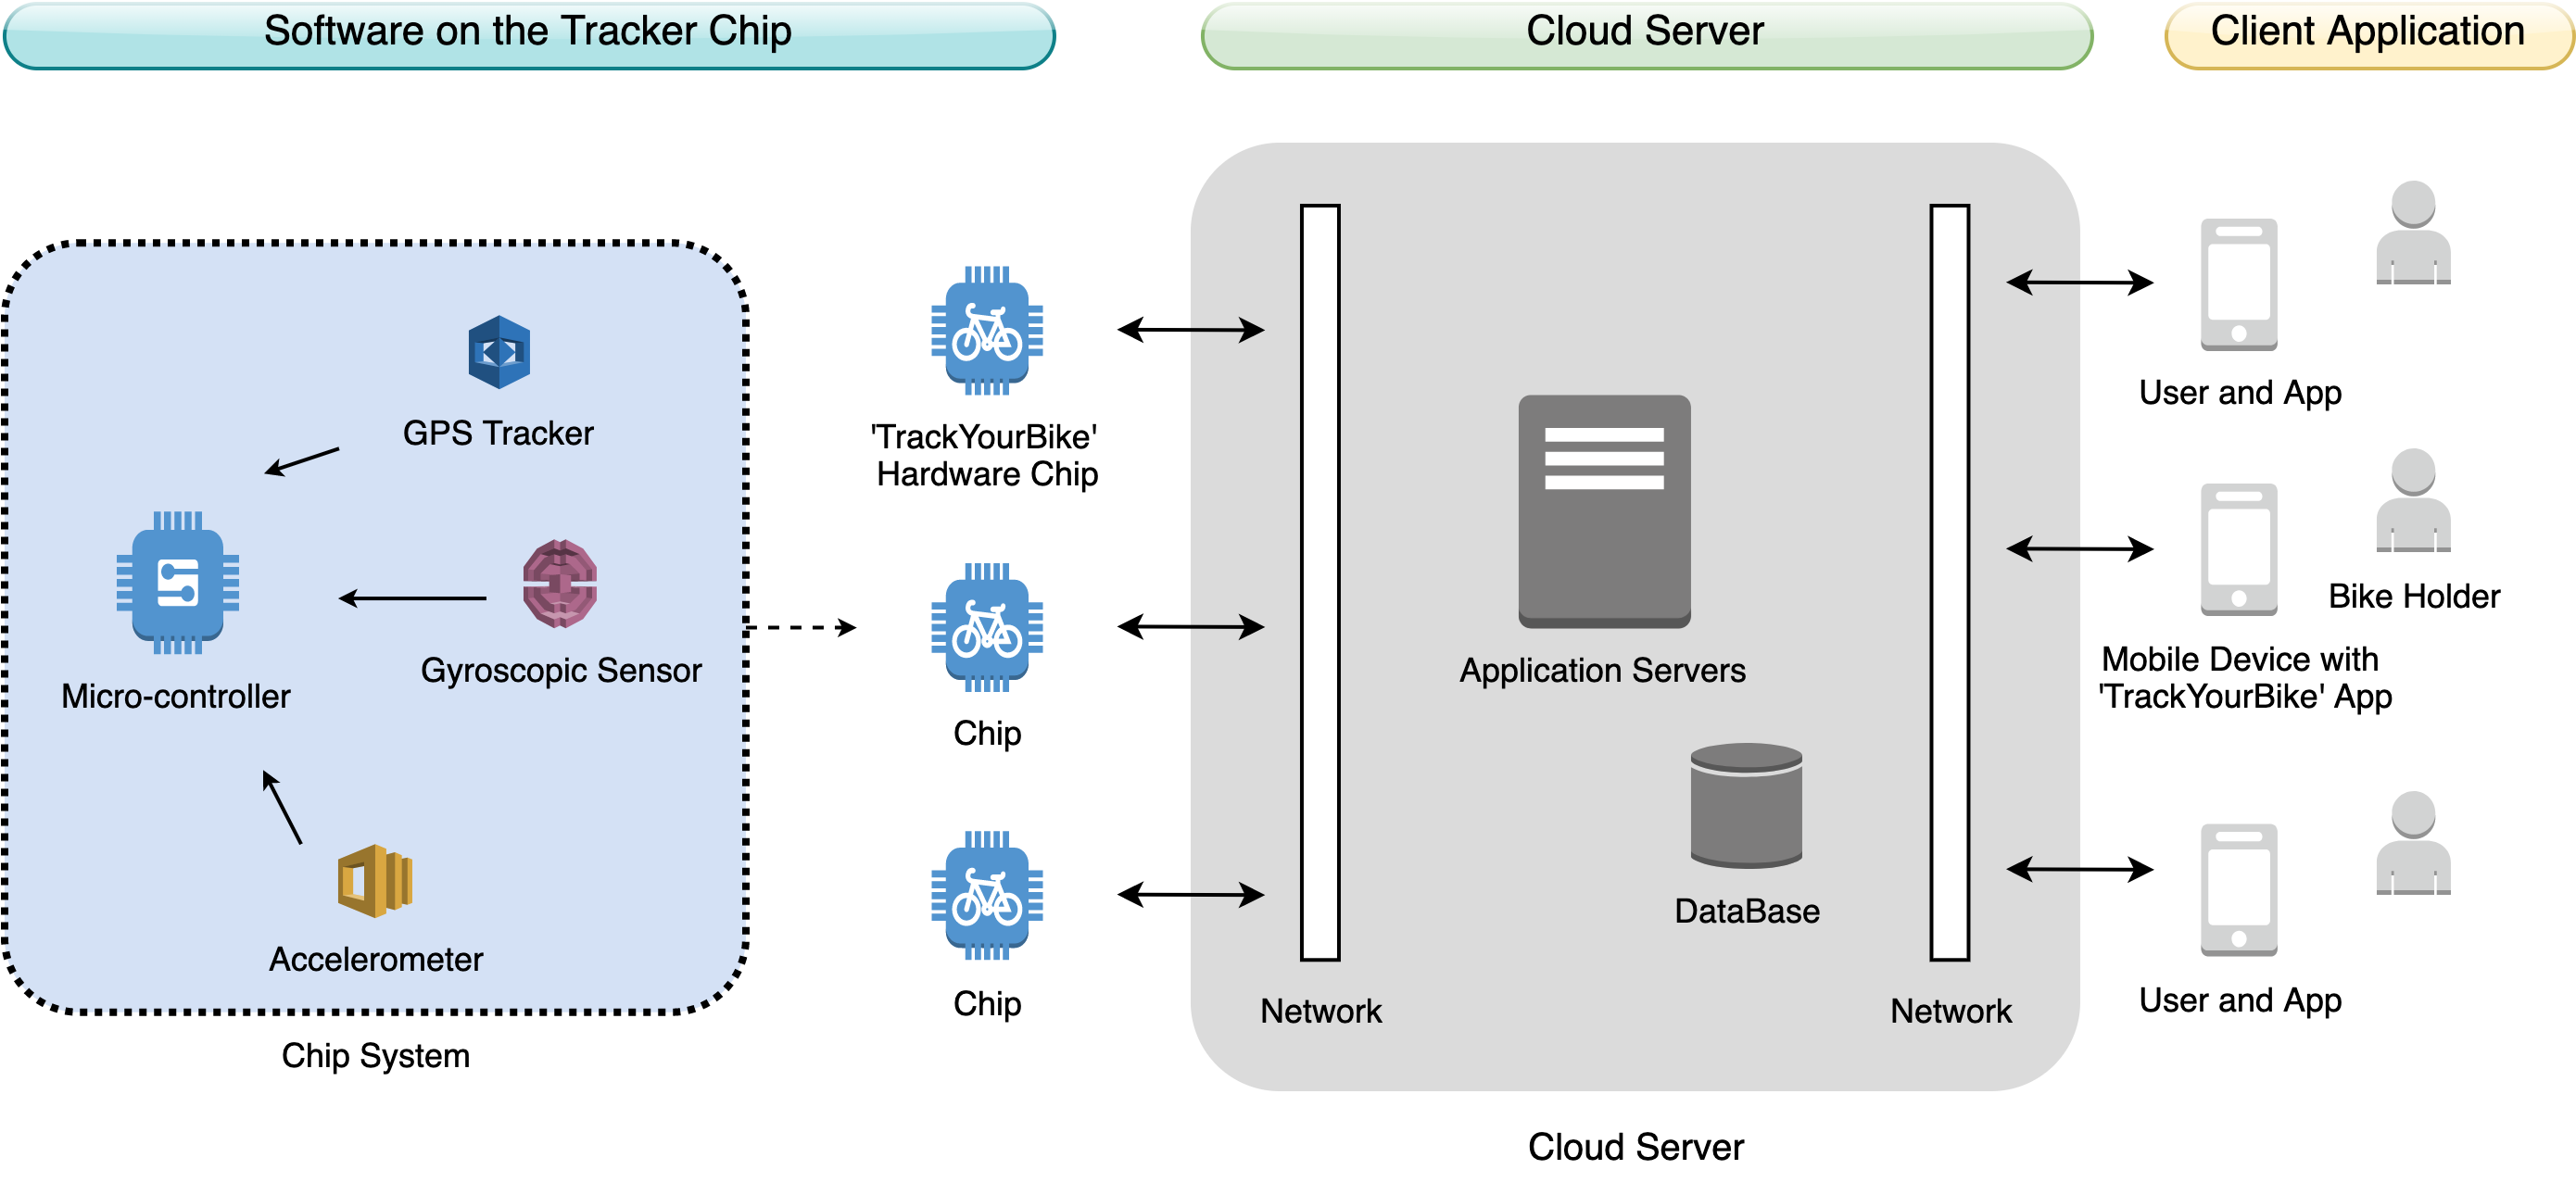
\includegraphics[width=0.8\textwidth]{./img/f2-sys-context.png}
	\caption{System Context Architecture}
	\label{fig:sys-context}
\end{figure}

\subsubsection*{\textbf{SRS for the Software on the Tracker Chip}}

Total of 4 SRS are defined for the \textit{Software on the Tracker Chip}.
In the scope of the assignment report, SRS 1, 2 and 3 are expanded with sub-requirements.

\begin{itemize}
	\item \textit{SRS 1.} The chip system shall receive the raw data sent from other sensors and adapt those raw data
	      into more structured data and send all structured data to the cloud server.
	      \begin{itemize}
		      \item [\textit{1.1}] \textit{Data Process Module:} this module shall handle the message construction part.
		            The module shall collect the raw data from 3 hardware components
		            and build them into a json format data.
		      \item [\textit{1.2}] \textit{Cloud Server Communication Module:} this module shall handle the communication part.
		            The module shall be able to receive message from the cloud server
		            and send json data described above to the server.
	      \end{itemize}

	\item \textit{SRS 2.} The chip system shall be able to receive a state data sent from the cloud server
	      which represents a state of \textit{Parked} and \textit{Unparked} and store this state into the memory of the micro-controller.
	      \begin{itemize}
		      \item [\textit{2.1}] \textit{State Management Module:} this module shall set the states described above into the chip.
	      \end{itemize}

	\item \textit{SRS 3.} The chip system shall be able to detect whether the bike is under the risk of stealing
	      based on the gyroscopic data.
	      \begin{itemize}
		      \item [\textit{3.1}] \textit{Risk Detection Module:} this module shall be able to estimate the risk level
		            based on the gyroscopic data.
	      \end{itemize}

	\item \textit{SRS 4.} The chip system shall sent a warning message to the cloud server to inform the user
	      that their bike is under the risk of stealing when the state is at \textit{Parked}.
\end{itemize}


\subsubsection*{\textbf{SRS for the Cloud Server System}}

\begin{itemize}
	\item \textit{Server-SRS 1.} The server system shall receive http request
	      and maintain socket connection with multiple clent-end.

	\item \textit{Server-SRS 2.} The system shall maintain the relationship between client-ends or hardware chips.

	\item \textit{Server-SRS 3.} The system shall receive chips data instantly and organize them into database,
	      and those data shall be analysed and pushed to the corresponding clent-end device.

	\item \textit{Server-SRS 4.} The system shall receive 'Parked' and 'Unparked' commands sent from a certain client-end
	      and associate them with the ressorted hardware chip instance.
\end{itemize}

\subsection*{\textbf{D3-System Design}}

\subsubsection*{\textbf{System Architectures}}

Fig. \ref{fig:sys-archs}\subref{fig:chip-sys-arch} depicts the \textit{Software on the Tracker Chip}'s top-down layer system architecture.
The top layer is dependent on the bottom layer in objects with vertical layer positions.
The grey box indicates that the objects do not have a hierarchy or layer relationship,
they are on the same architectural level.

% A top-down layer system architecture of the \textit{Software on the Tracker Chip} is shown in Fig. \ref{fig:chip-sys-arch}.
% The objects with vertical layer position mean that the top layer depends on the bottom layer.
% Notice that the obejcts in the gray box mean that they do not have hierarchy or layer relationship, they are in the same architecture level.

% \begin{figure}[!ht]
% 	\centering
% 	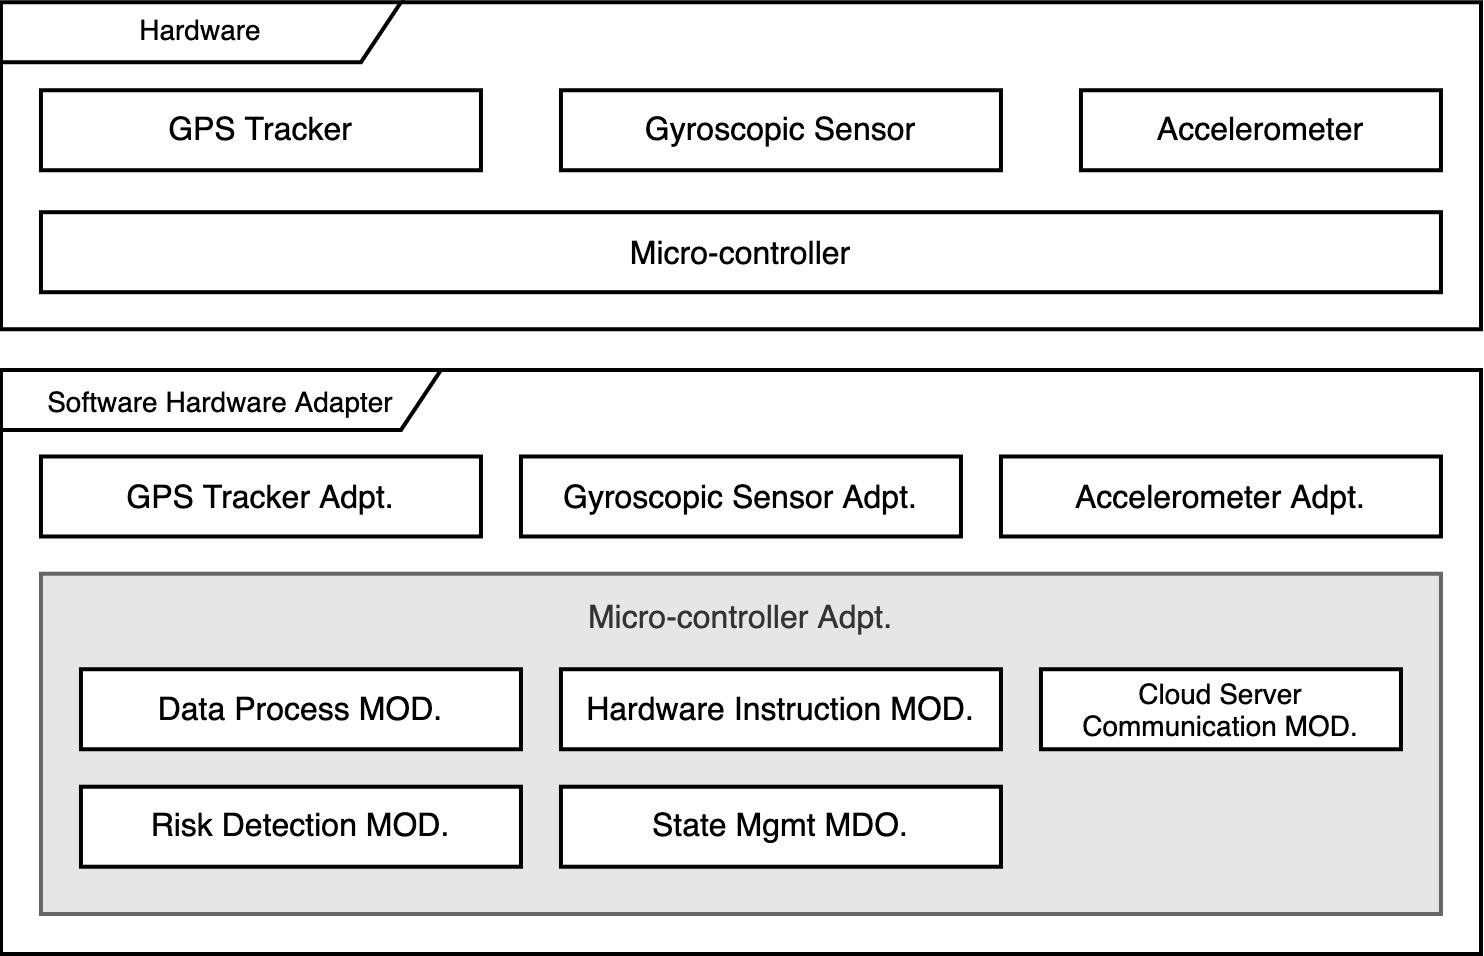
\includegraphics[width=0.6\textwidth]{./img/f3-chip-sys-architecture.png}
% 	\caption{Architecture of the \textit{Software on the Tracker Chip}}
% 	\label{fig:chip-sys-arch}
% \end{figure}

Then a same top-down layer system architecture of the \textit{Cloud Server System} is shown in Fig \ref{fig:sys-archs}\subref{fig:cloud-sys-arch}.

% \begin{figure}[!ht]
% 	\centering
% 	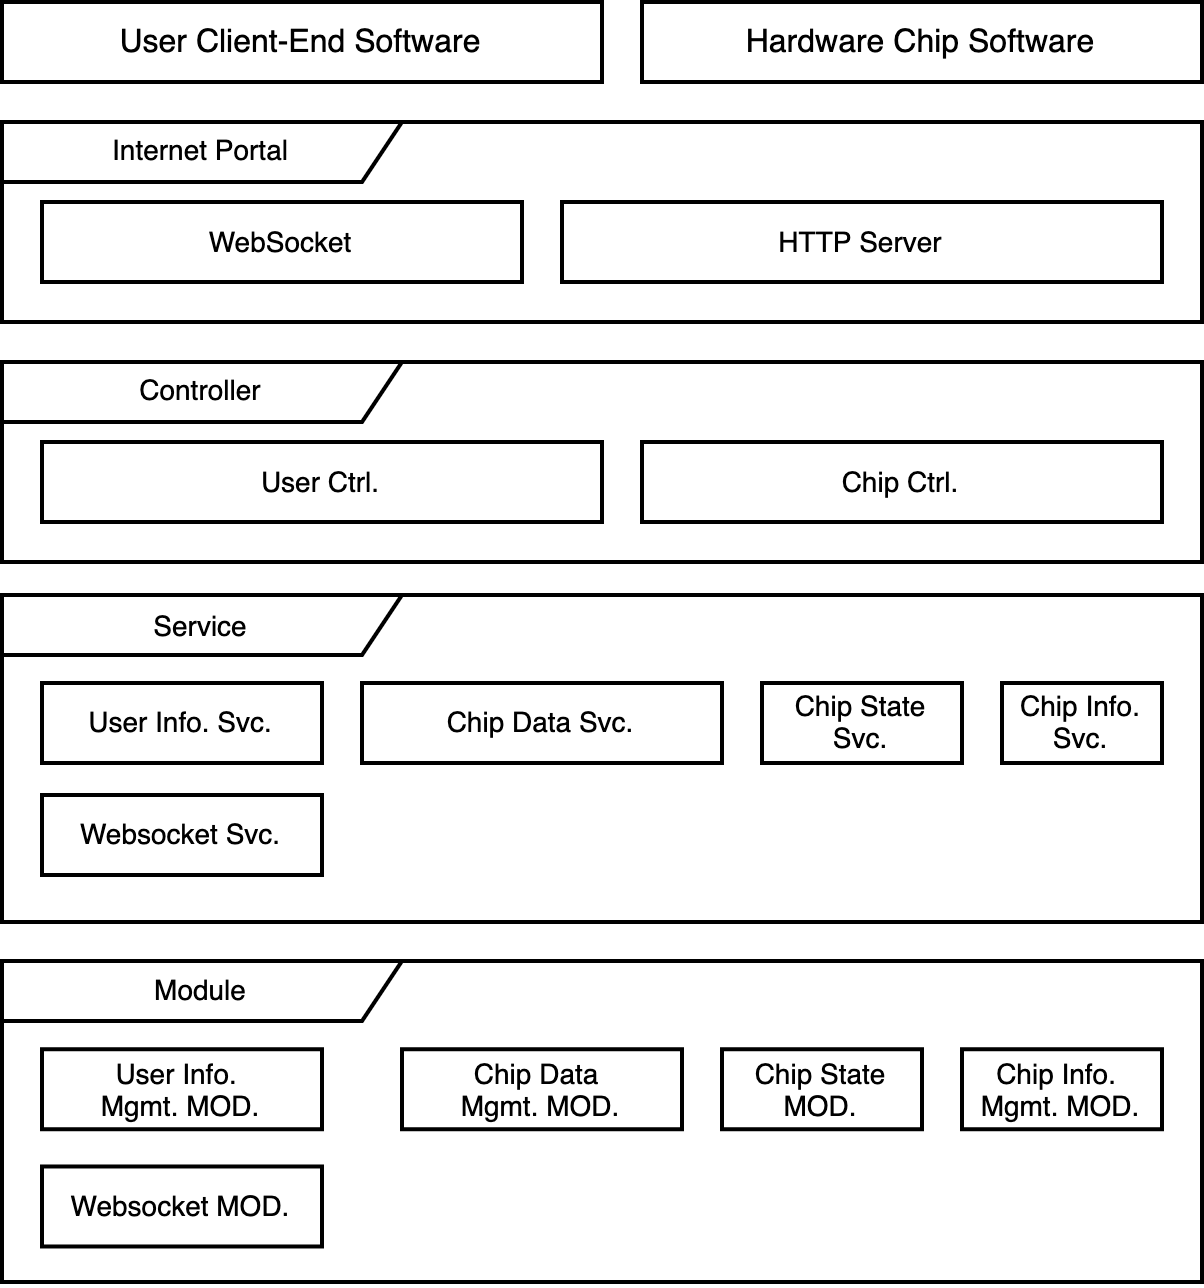
\includegraphics[width=0.6\textwidth]{./img/f4-cloud-sys-architecture.png}
% 	\caption{Architecture of the \textit{Cloud Server System}}
% 	\label{fig:cloud-sys-arch}
% \end{figure}

\begin{figure*}[!ht]
	\centering
	\subfloat[Architecture of the \textit{Software on the Tracker Chip}]
	{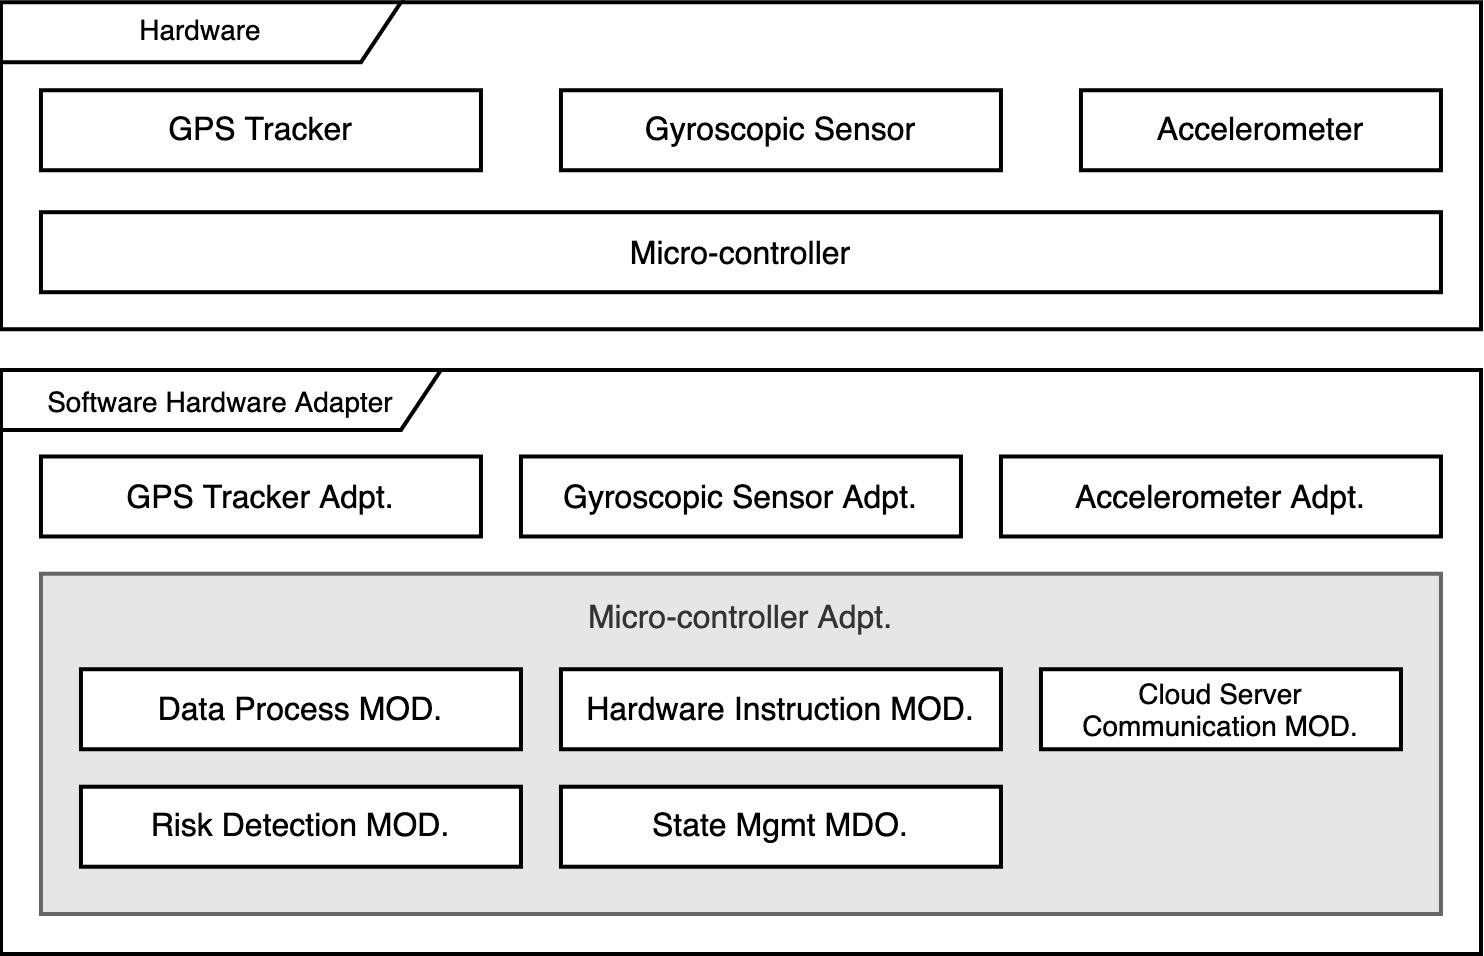
\includegraphics[width=3.8in, valign=m]{./img/f3-chip-sys-architecture.png}\label{fig:chip-sys-arch}}
	\hfil
	\hspace{0.2in}
	\subfloat[Architecture of the \textit{Cloud Server System}]
	{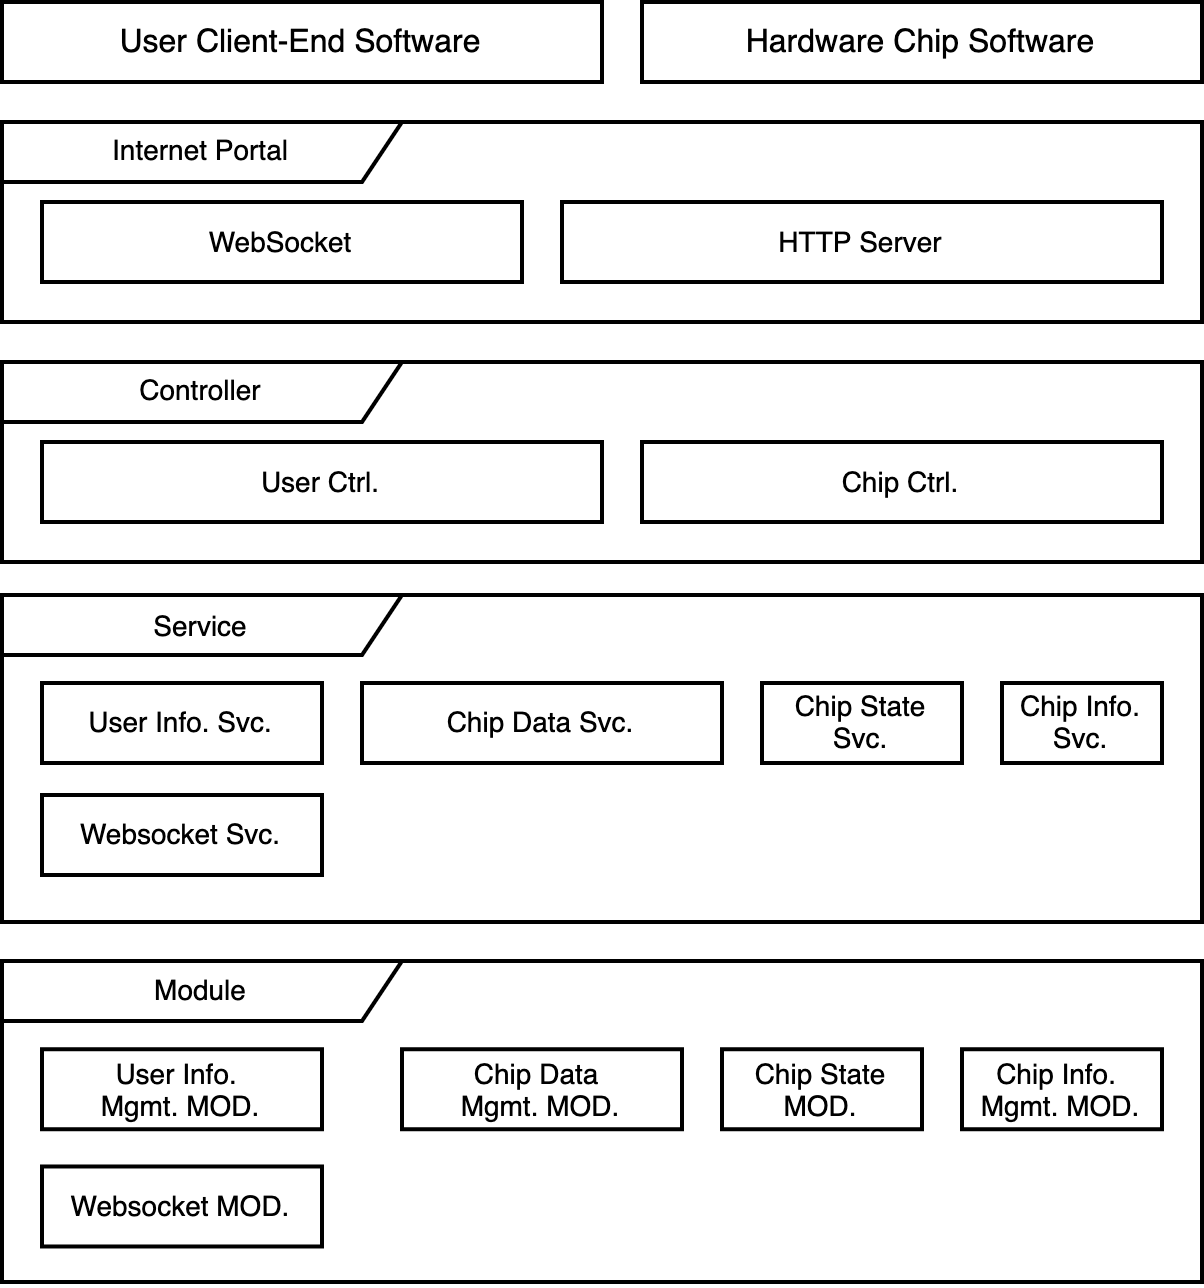
\includegraphics[width=3in, valign=m]{./img/f4-cloud-sys-architecture.png}\label{fig:cloud-sys-arch}}
	% \caption{System Architectures}
	\caption{
		System Architectures:
		\protect\subref{fig:chip-sys-arch}
		\protect\subref{fig:cloud-sys-arch}
	}
	\label{fig:sys-archs}
\end{figure*}


\subsubsection*{\textbf{Activitiy Diagram of Some Key Processes on the \textit{Software on the Tracker Chip}}}

The activity diagrems are shown in Fig. \ref{fig:activity-diagram}.

\begin{figure*}[!ht]
	\centering
	\subfloat[Activitiy Diagram of SRS 1, 3, and 4]{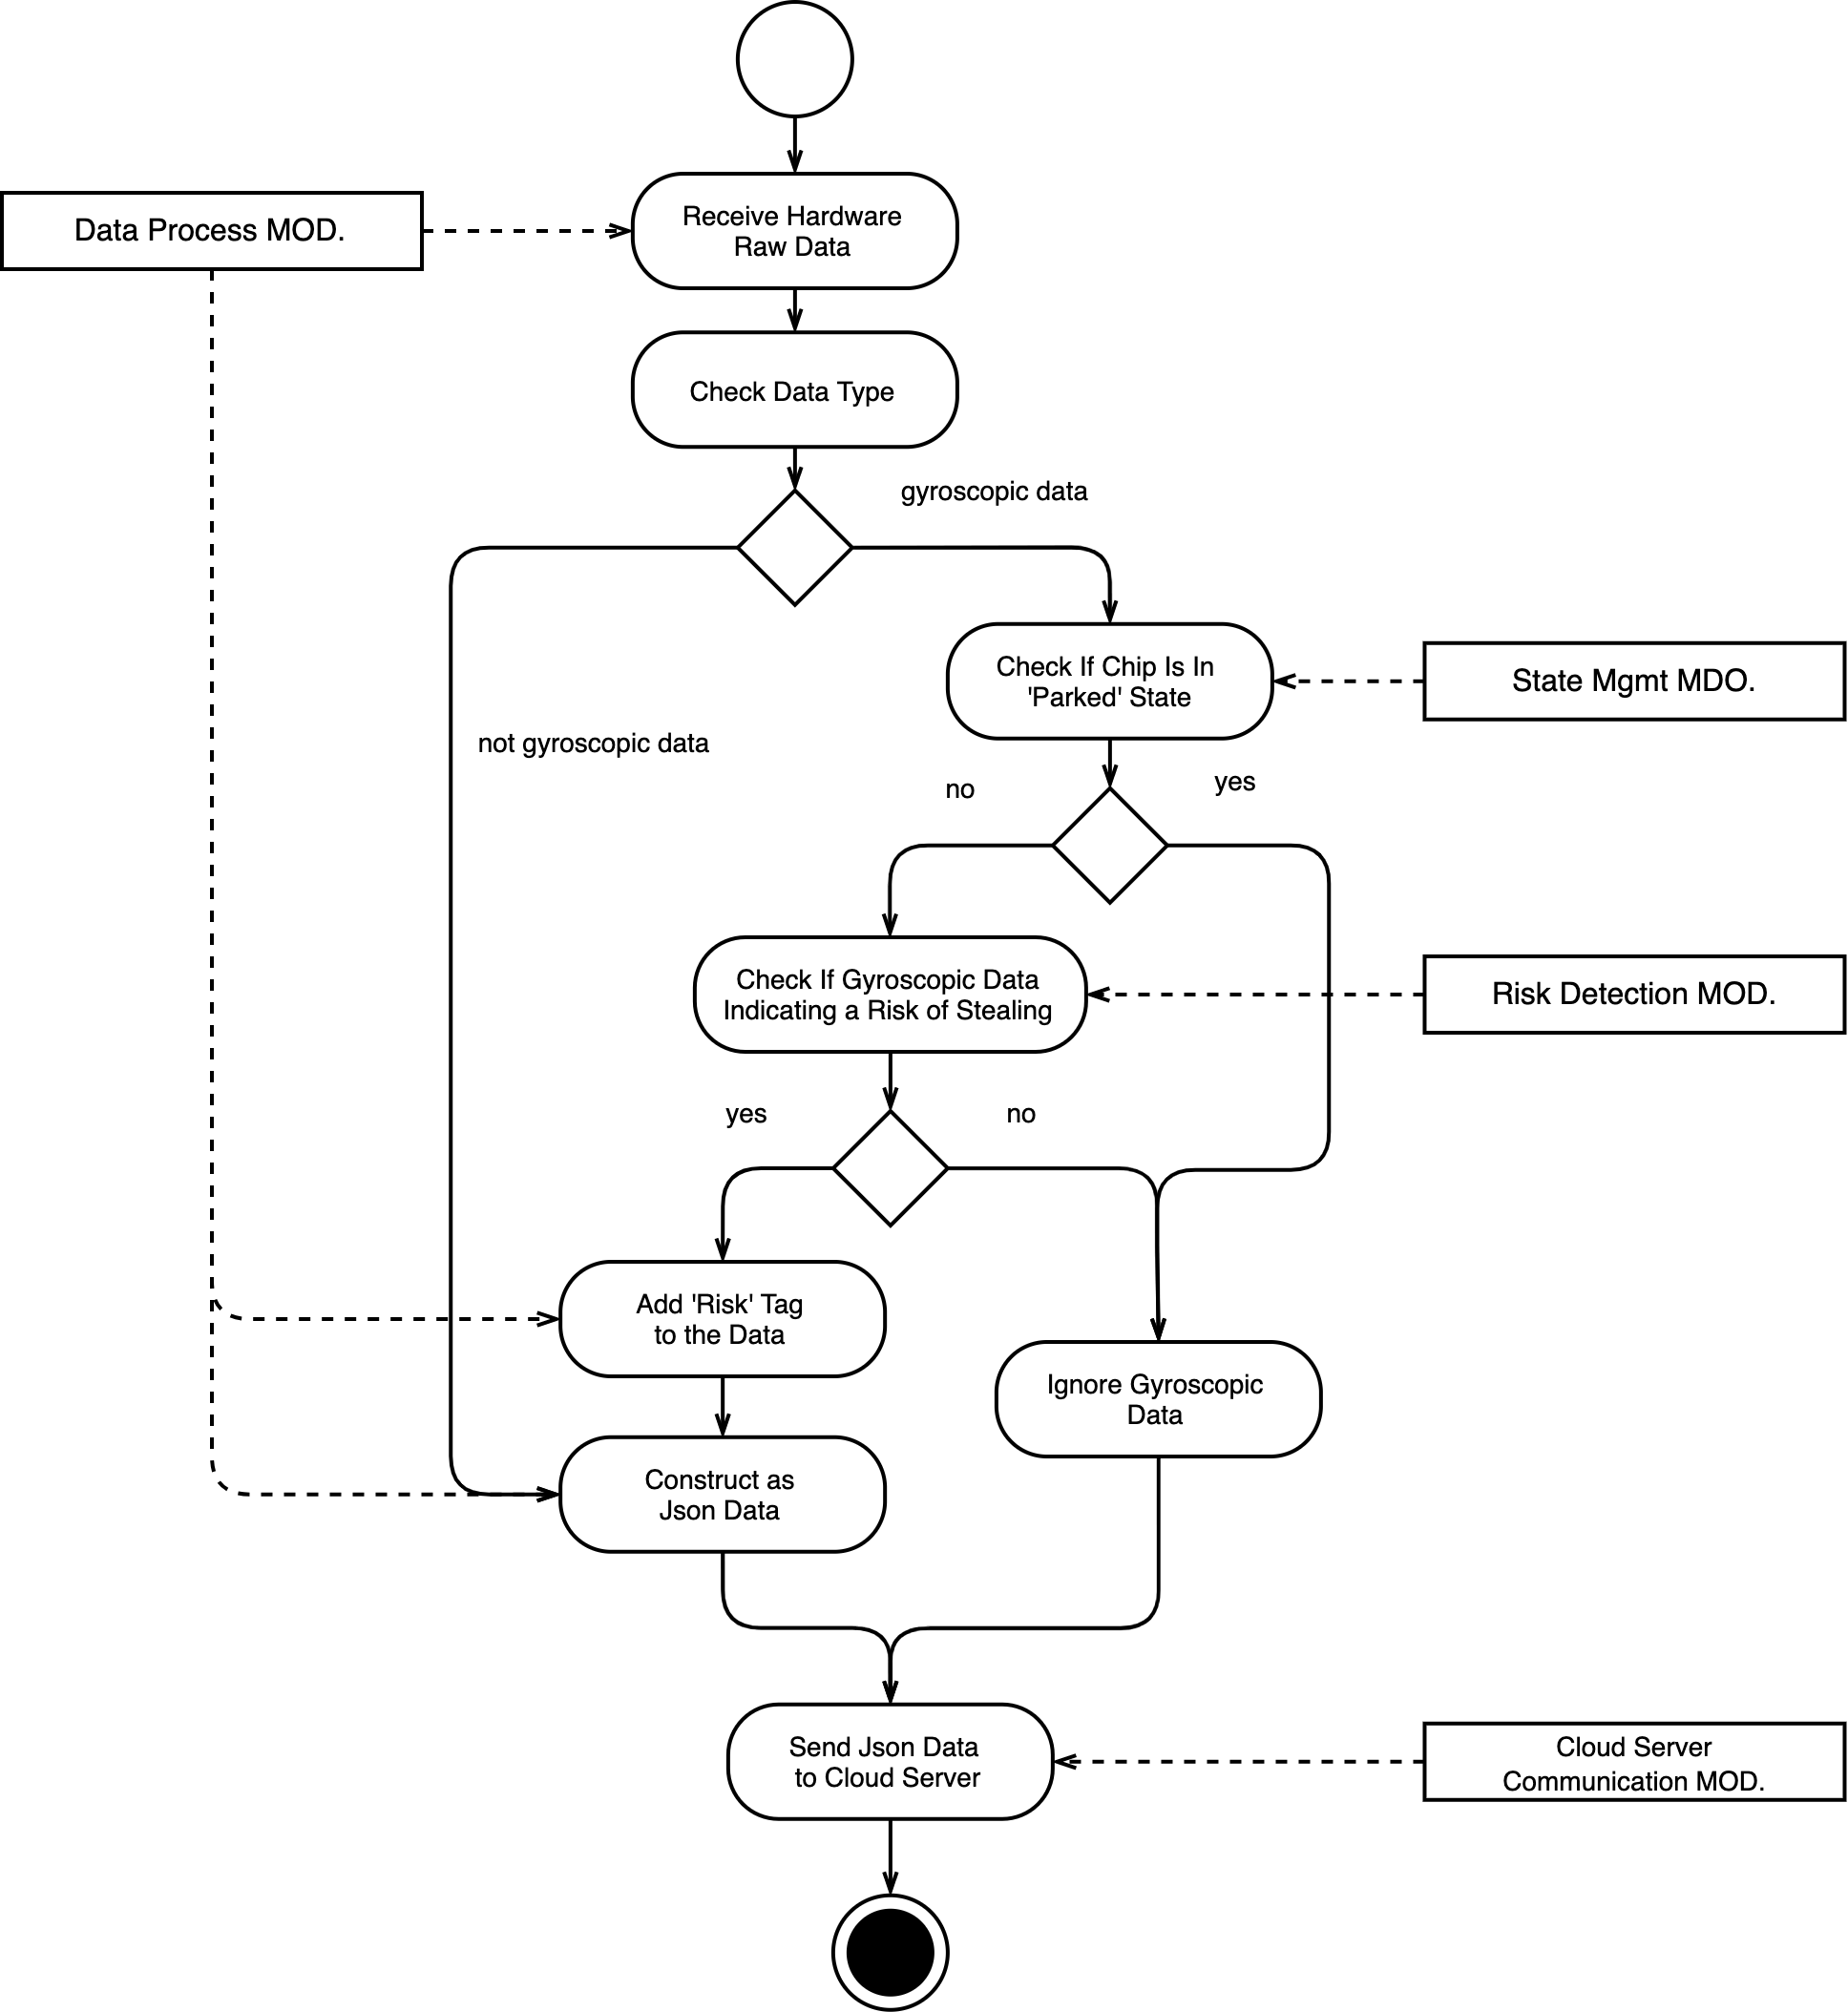
\includegraphics[width=3.8in, valign=m]{./img/f5-activity-diagram-1.png}
		\label{fig:ad-1}}
	\hfil
	\hspace{0.2in}
	\subfloat[Activitiy Diagram of SRS 2]{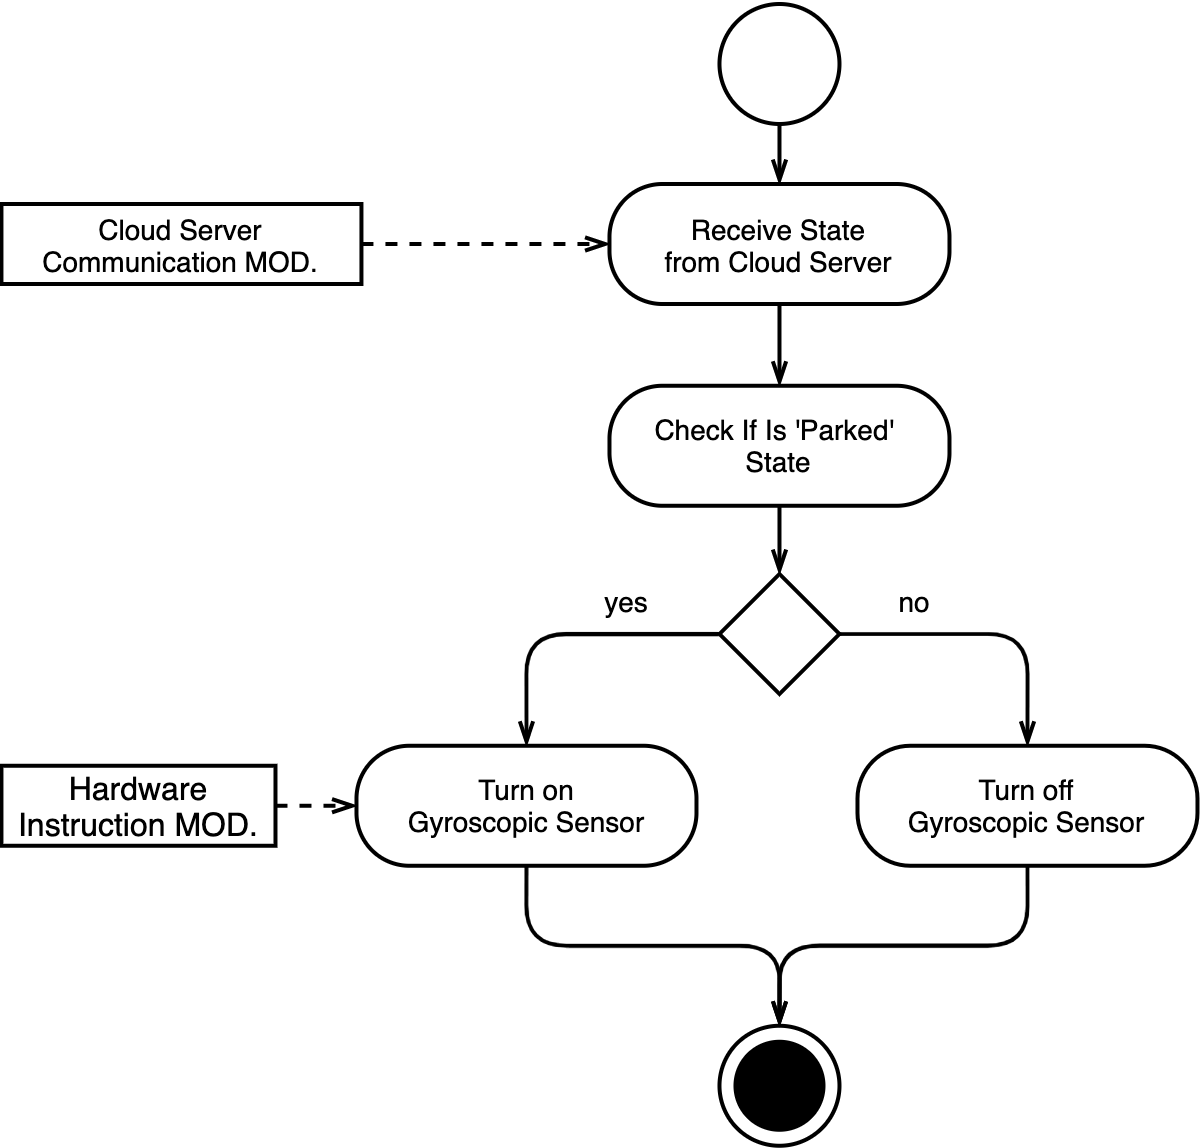
\includegraphics[width=3in, valign=m]{./img/f6-activity-diagram-2png.png}
		\label{fig:ad-2}}
	\caption{Activity Diagrams of the SRS}
	\label{fig:activity-diagram}
\end{figure*}

\subsection*{\textbf{D4-Define An Incremental Process}}

The defined incremental process is shown in Fig. \ref{fig:incre-process}.
The process is consist of the techniques like \textquote{Incremental Planning} and
\textquote{Test First Development} from the \textit{Extreme Programming}.

To perform the incremental process, a loop starts at step 4
and ends with step 7 when no unfinished tasks are left on the storyboard.
Every task will start from defining the test cases and then developing and validating.

SRS 2 is chosen to practice the incremental process with XP methodologies.

\begin{figure}[!ht]
	\centering
	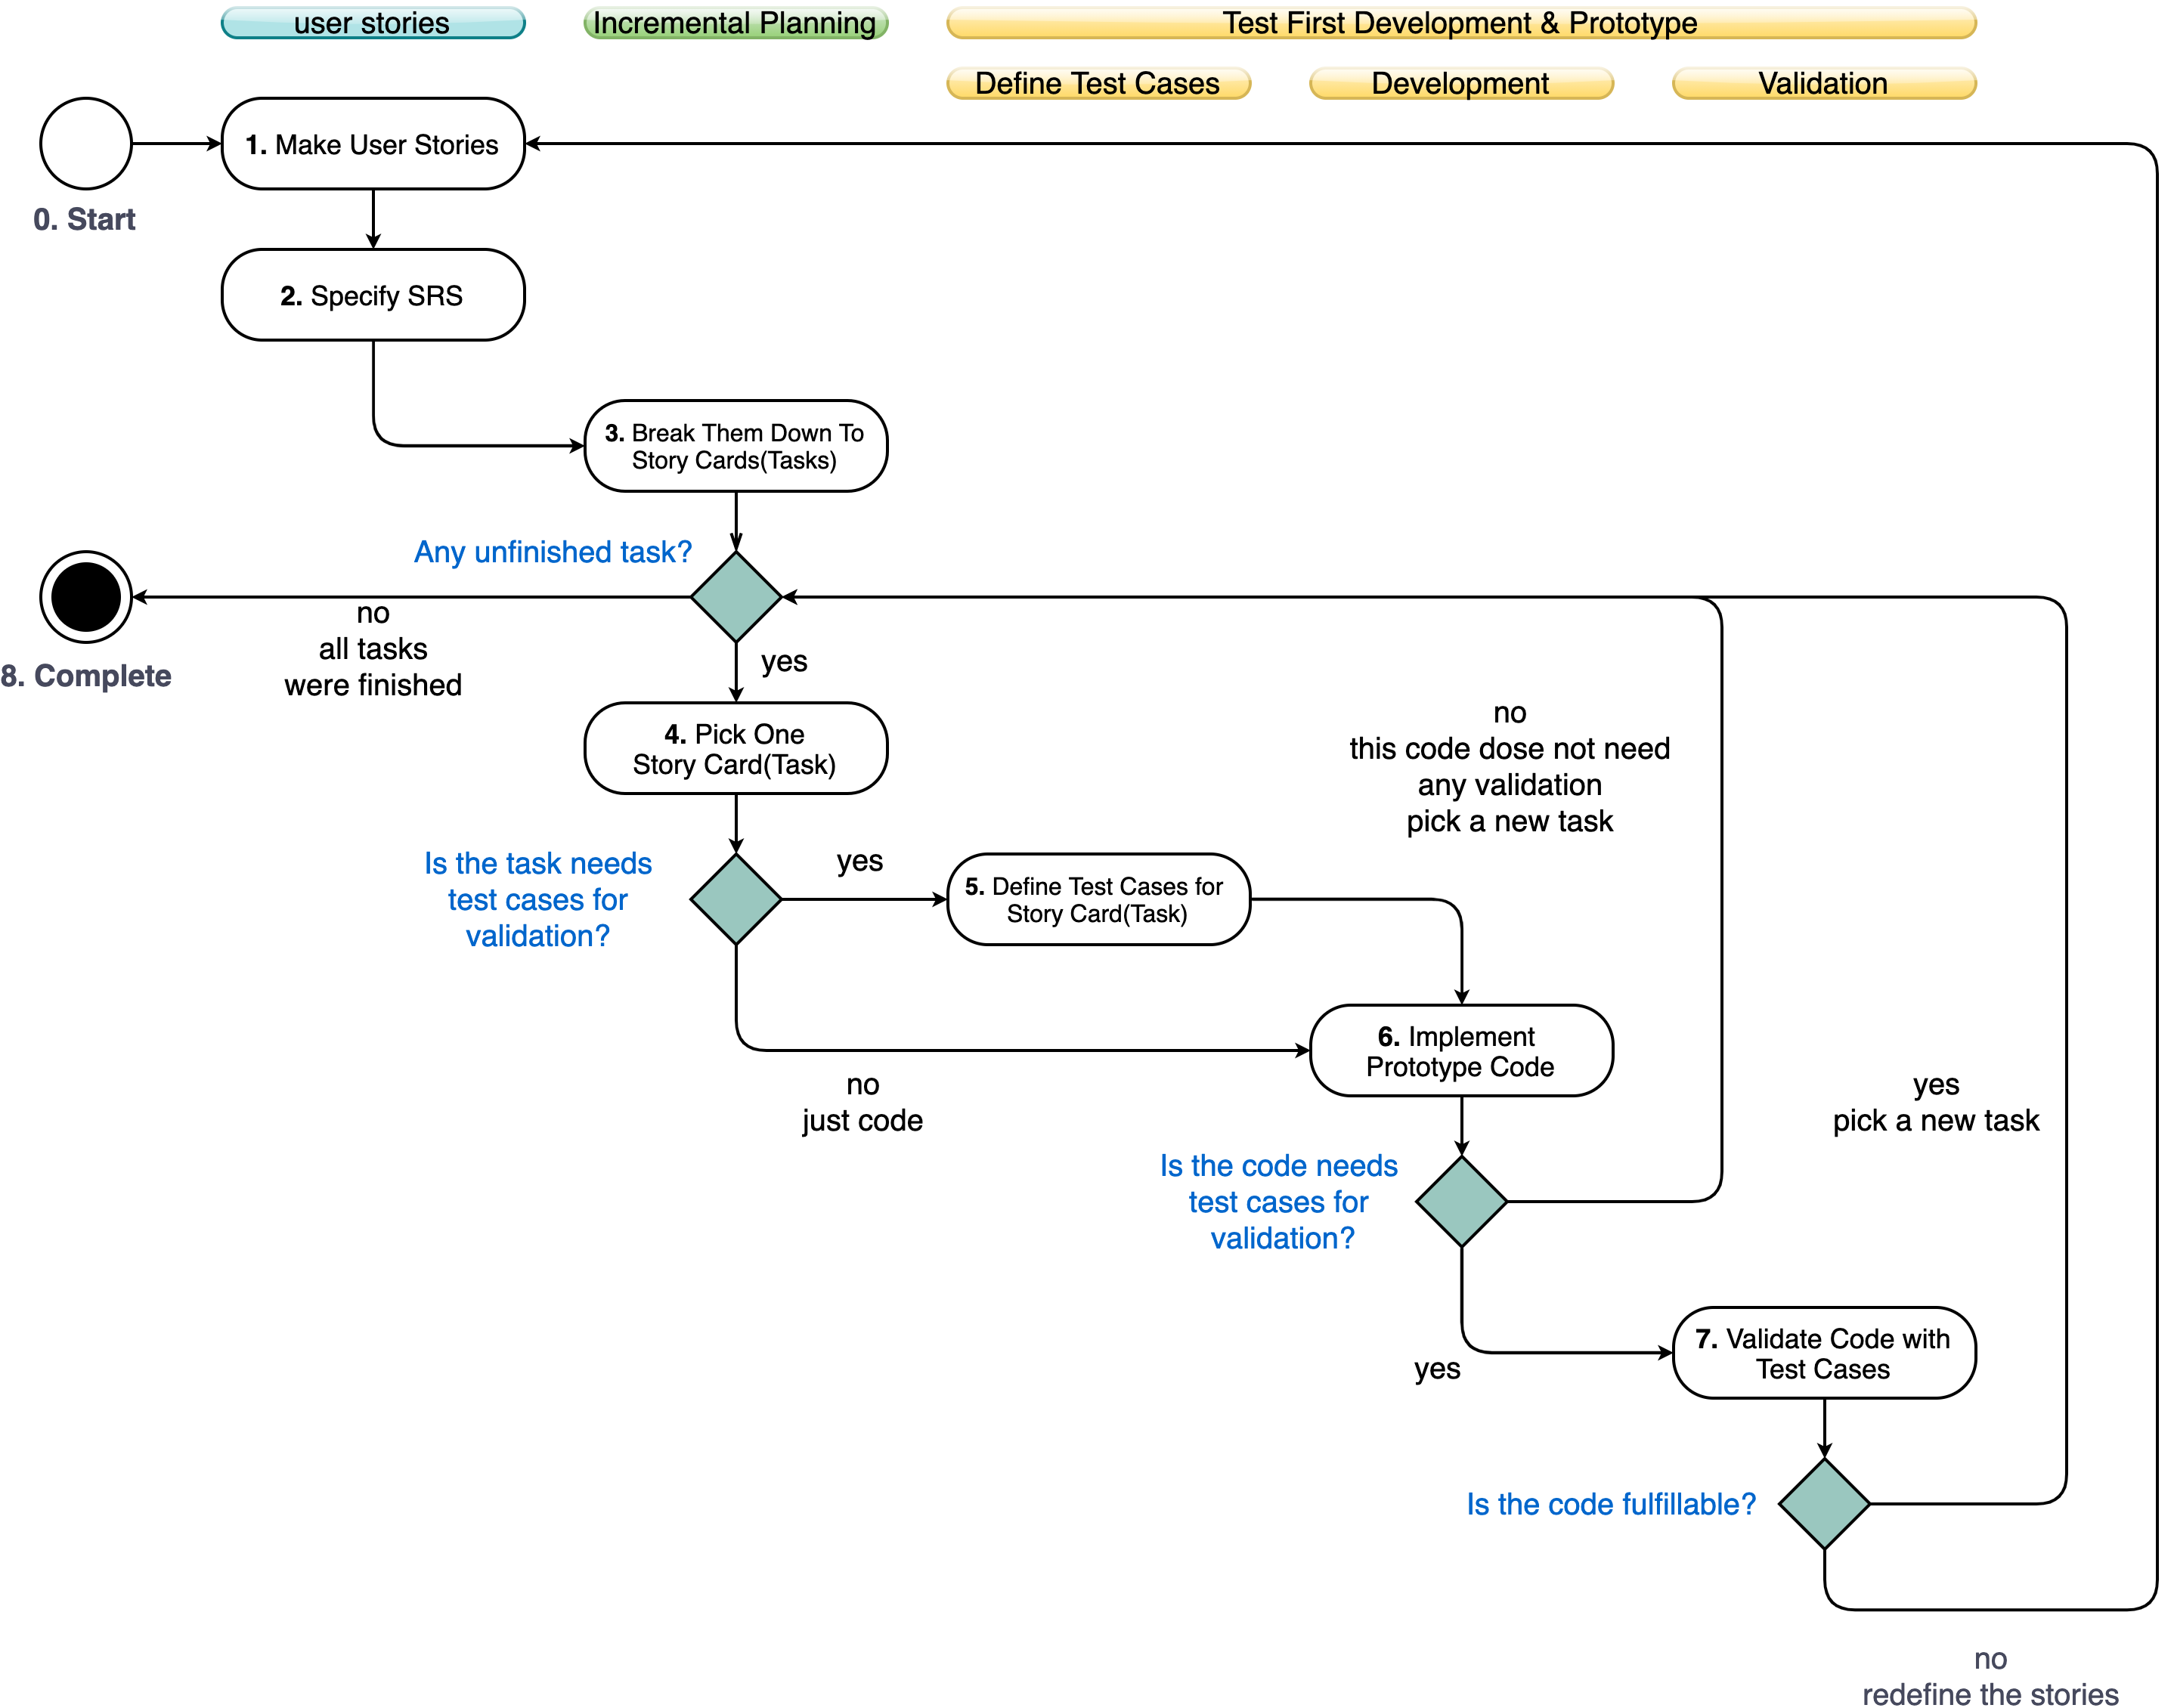
\includegraphics[width=0.9\textwidth]{./img/f7-incremental-process.png}
	\caption{Incremental Process}
	\label{fig:incre-process}
\end{figure}

\subsection*{\textbf{D5-Practice with the Extreme Programming}}

\subsubsection*{\textbf{Story Cards}}

Following the \textit{Incremental Planning} technique,
SRS 2 can be partitioned as several story cards(tasks) which are shown in Table \ref{tb:1}.

\begin{table}[!ht]
	\renewcommand{\arraystretch}{1.5}
	\caption{Story Cards(Tasks) of SRS 2}
	\label{tb:1}
	\centering
	\begin{tabular}{l | L{3cm} | L{3cm} | L{5cm}}
		\hline
		\textbf{No.Title}    & \textbf{0. Mock Raw Data}                                                         & \textbf{1. Data Class Definition}           & \textbf{2. Build Raw Data into Json Data}             \\
		\hline
		\textbf{Description} & Mock the raw data which sent from the hareware sensors for unit test verification & Define classes which represent the raw data & A module to construct the raw data into the Json Data \\
		\hline
	\end{tabular}
\end{table}

\subsubsection*{\textbf{Finish the Task}}

\textit{Task 1} is chosen to be presented in this report.
However, mocked sensor raw data is required for the unit test.
With the mock data, the console of the IDE will represent the display device
that the client will use, and all raw data will be reconstructed to json data.
This implies that the task result will be validated manually by observing the console.

\newpage
\textbf{Task 0}

\textit{Task 0} started first. As can be seen in Fig. \ref{fig:task0-testcase},
the code will generate one raw data record of the GPS tracker. So as the raw data of accelerometer and the gyroscopic sensor.
The code will be located in \textquote{src/test/java/io/github/youyinnn/bo/chip/RawDataMocker.java}.

\begin{figure}[!ht]
	\centering
	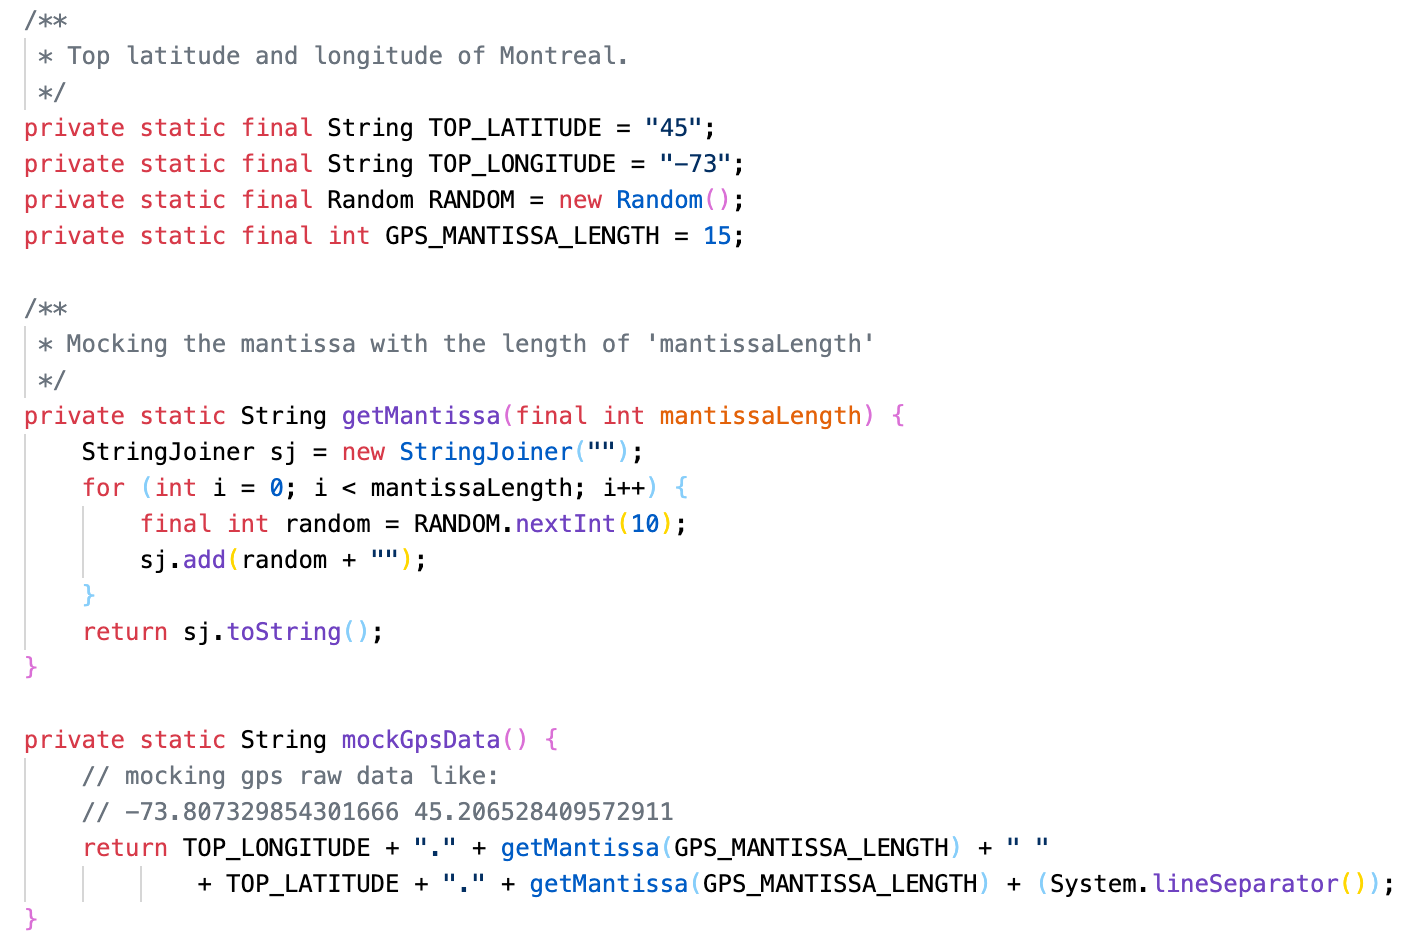
\includegraphics[width=0.65\textwidth]{./img/f8-task0-testcase.png}
	\caption{Test Cases of Generating Raw Data of GPS Tracker}
	\label{fig:task0-testcase}
\end{figure}

In the first loop, the raw data did not contain the timestamp, so the test cases are not fulfilled
since those data are displayed in a real-time situation.
As the result, a second loop was started, and the incremental code is presented in Fig. \ref{fig:incre-code-1}.

\begin{figure}[!ht]
	\centering
	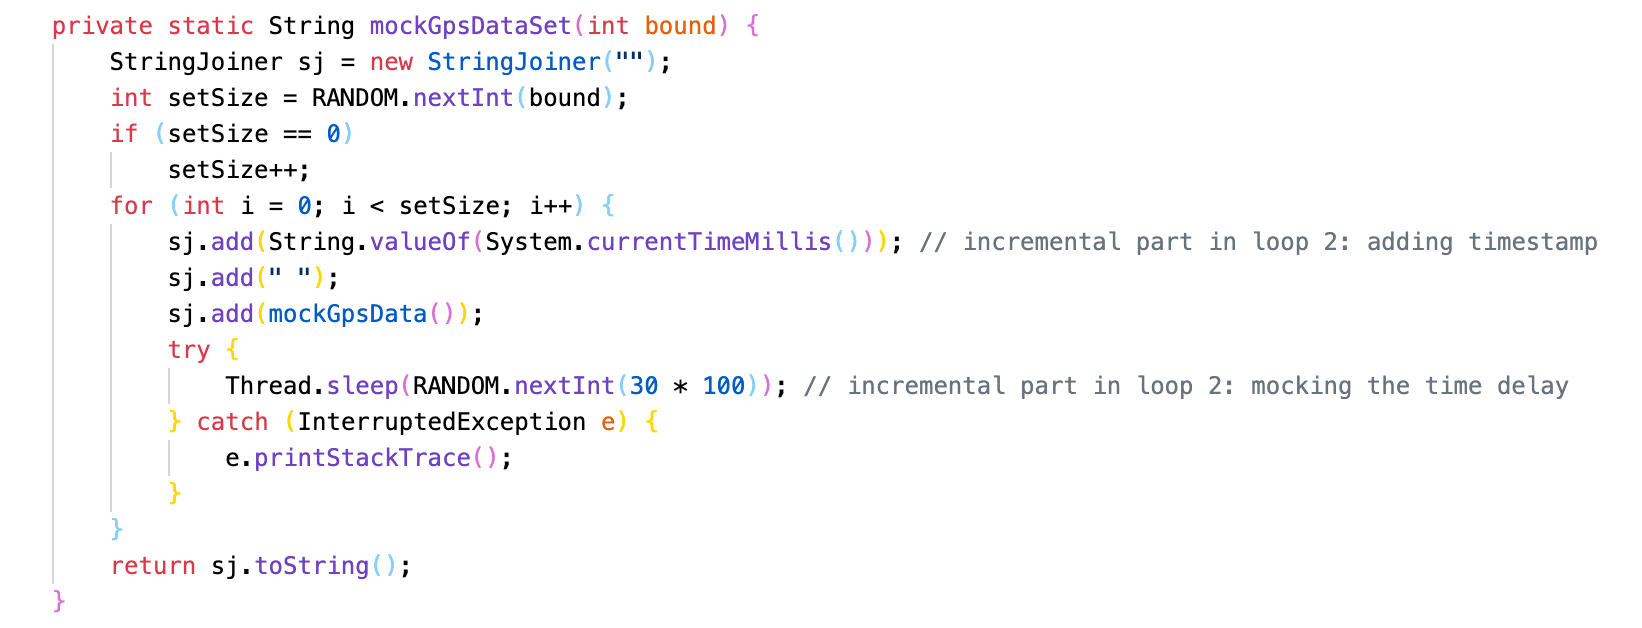
\includegraphics[width=0.8\textwidth]{./img/f12-incremental-code-1.png}
	\caption{Revised Code which Generating Timestamp before the Raw Data}
	\label{fig:incre-code-1}
\end{figure}

The revised sample of the raw data is shown in \ref{fig:raw-data-sample}.
Those data samples are located in \textquote{src/main/resources/data\_samples}.


\textbf{Task 1}

\begin{itemize}
	\item \textbf{Test Cases:} The test cases for task 1 can be defined as Fig. \ref{fig:test-code-t1} is shown.
	      Its location is \textquote{src/test/java/io/github/youyinnn/module/chip/ChipDataProcessorImplTest.java}.

	\item \textbf{Code Implementation:} After test cases defined, then the implementation of the \textit{ChipDataProcessor} was implemented
	      which is \textit{ChipDataProcessorImpl} and is shown in Fig. \ref{fig:intf-impl}.
	      The corresponding class diagrams of the data objects are shown in Fig. \ref{fig:class-diagram}.
	      And their implementations are located in \textquote{src/main/java/io/github/youyinnn/bo/chip}.

	\item \textbf{Validation:} After all the implementations were done, the test units were executed
	      and they were all passed(shown in Fig. \ref{fig:test-result}).
	      This means the task 1 was completed and the loop for this task was finished.
\end{itemize}

\begin{figure}[!ht]
	\centering
	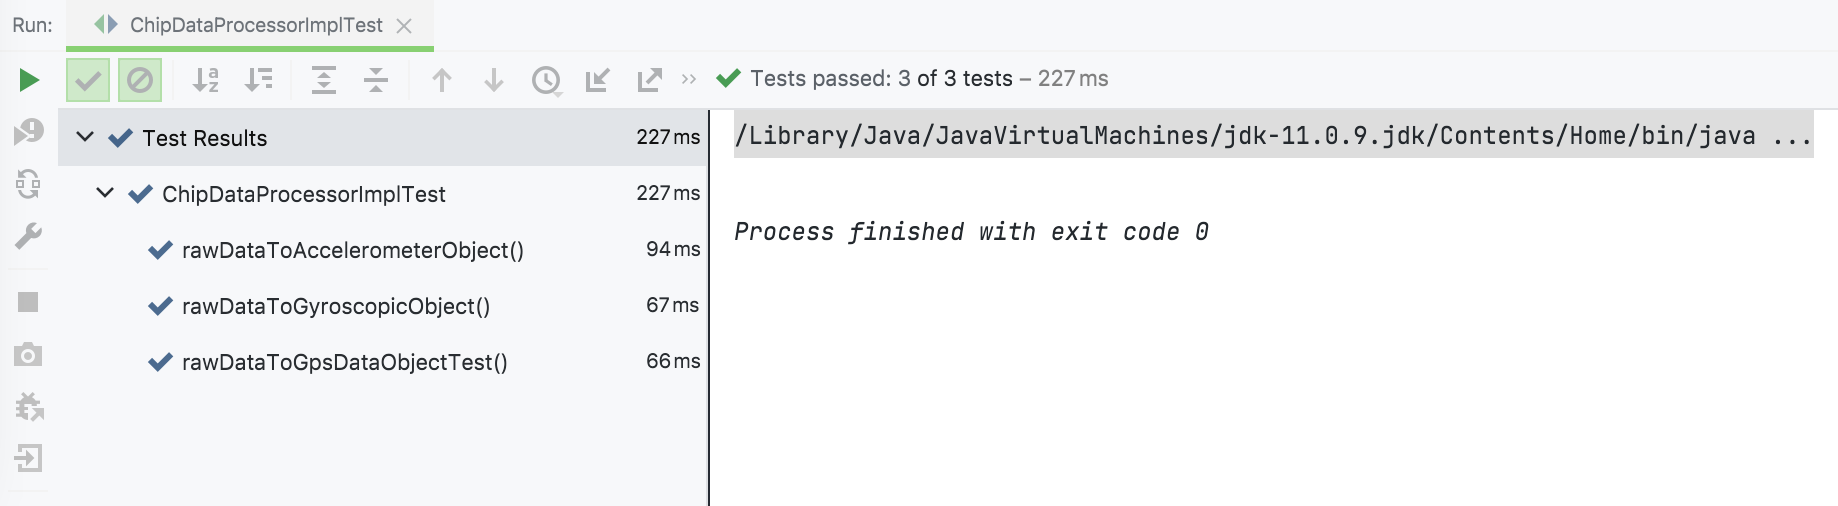
\includegraphics[width=0.8\textwidth]{./img/f19-t1-test-result.png}
	\caption{Result of the Unit Test of Task 1}
	\label{fig:test-result}
\end{figure}

\begin{figure*}[!ht]
	\centering
	\subfloat[Raw Data of GPS Tracker]{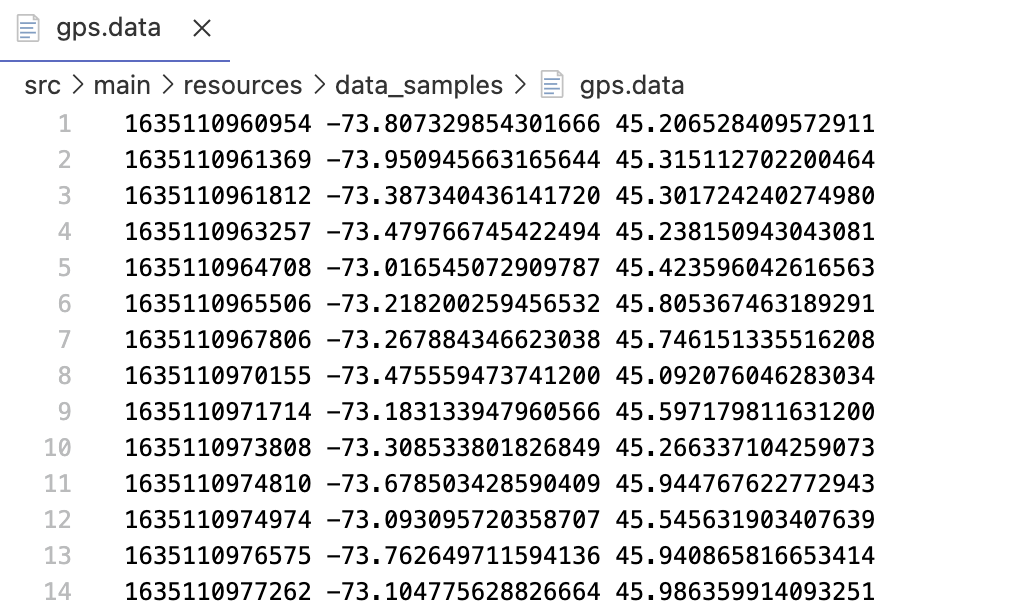
\includegraphics[width=3.3in, valign=m]{./img/f9-gps-data-sample.png}
		\label{fig:gps-data}}
	\hfil
	\hspace{0.2in}
	\subfloat[Raw Data of Accelerometer]{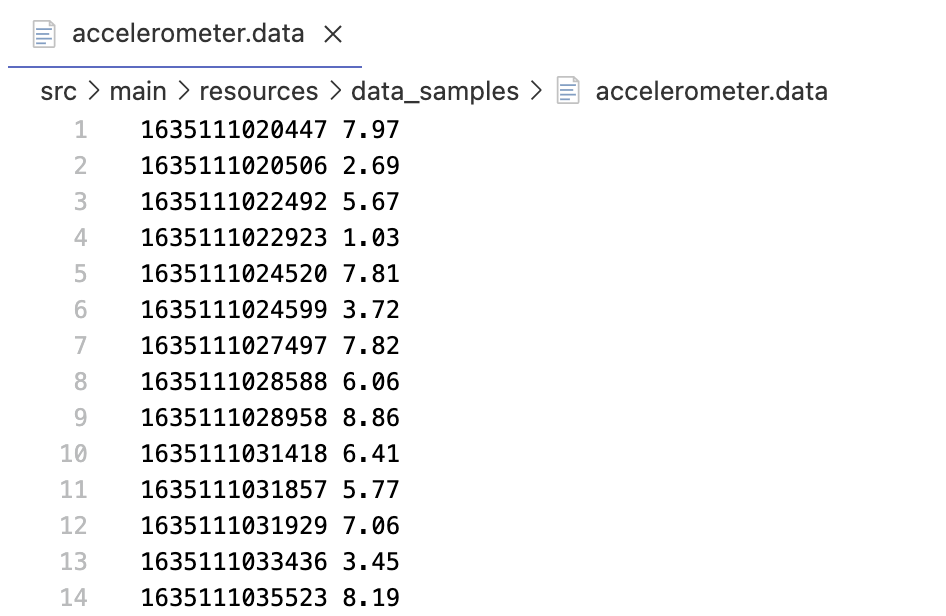
\includegraphics[width=3in, valign=m]{./img/f10-speed-data-sample.png}
		\label{fig:speed-data}}
	\vspace{0.2in}
	\subfloat[Raw Data of Gyroscopic Sensor]{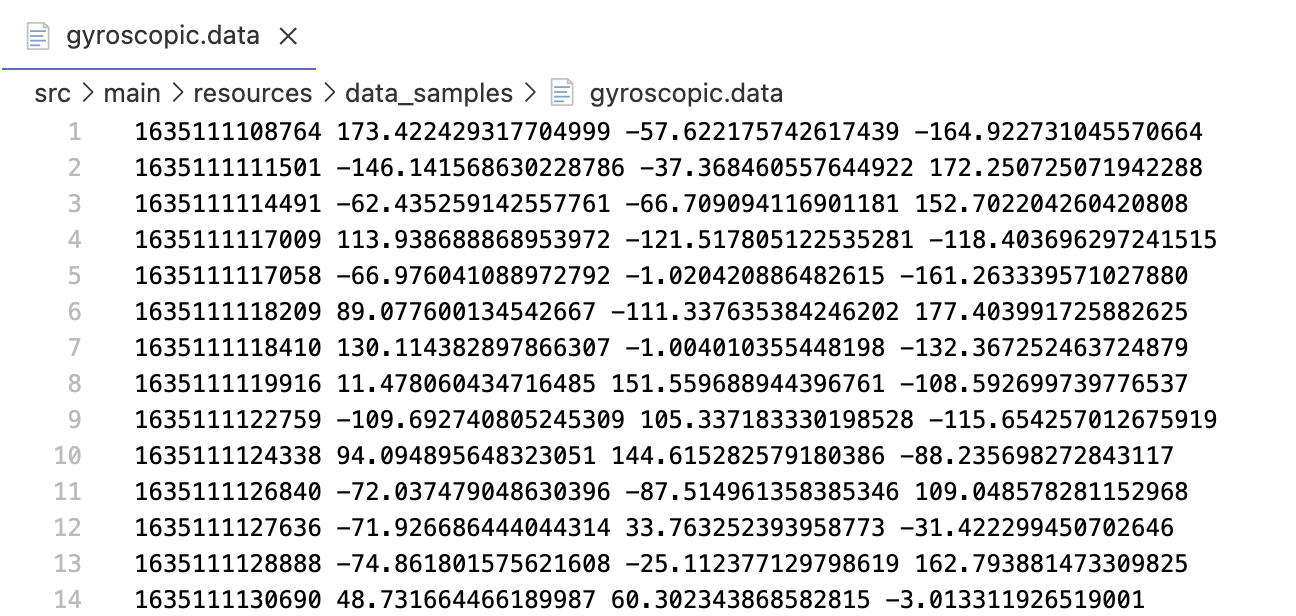
\includegraphics[width=3.8in, valign=m]{./img/f11-gyroscopic-data-sample.png}
		\label{fig:gy-data}}
	\caption{Mocked Raw Data}
	\label{fig:raw-data-sample}
\end{figure*}

\begin{figure}[!htp]
	\centering
	\subfloat[\textit{ChipDataProcessor} Interface]{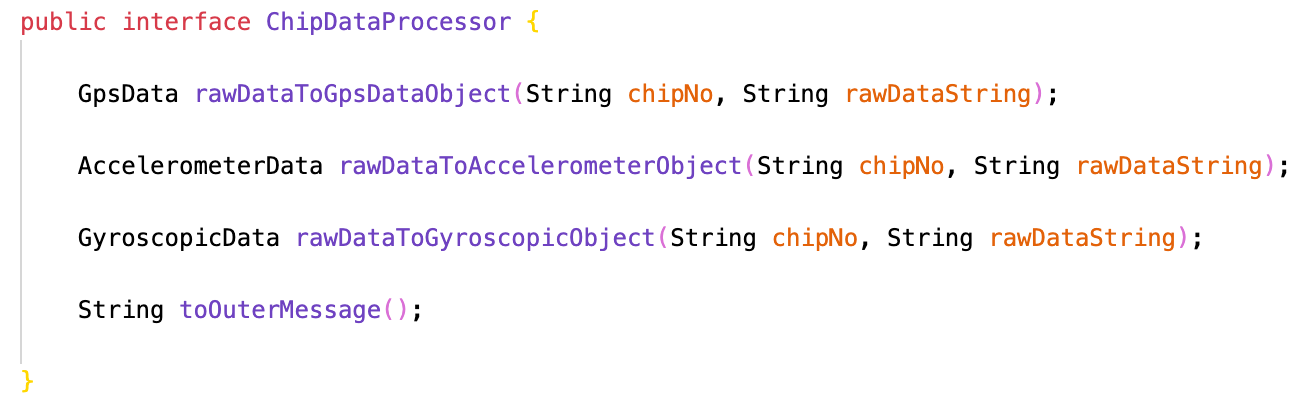
\includegraphics[width=4in, valign=m]{./img/f16-t1-testcase-4-intf.png}
		\label{fig:t1-intf}}
	\hfil
	\subfloat[Preparing the Raw Data]{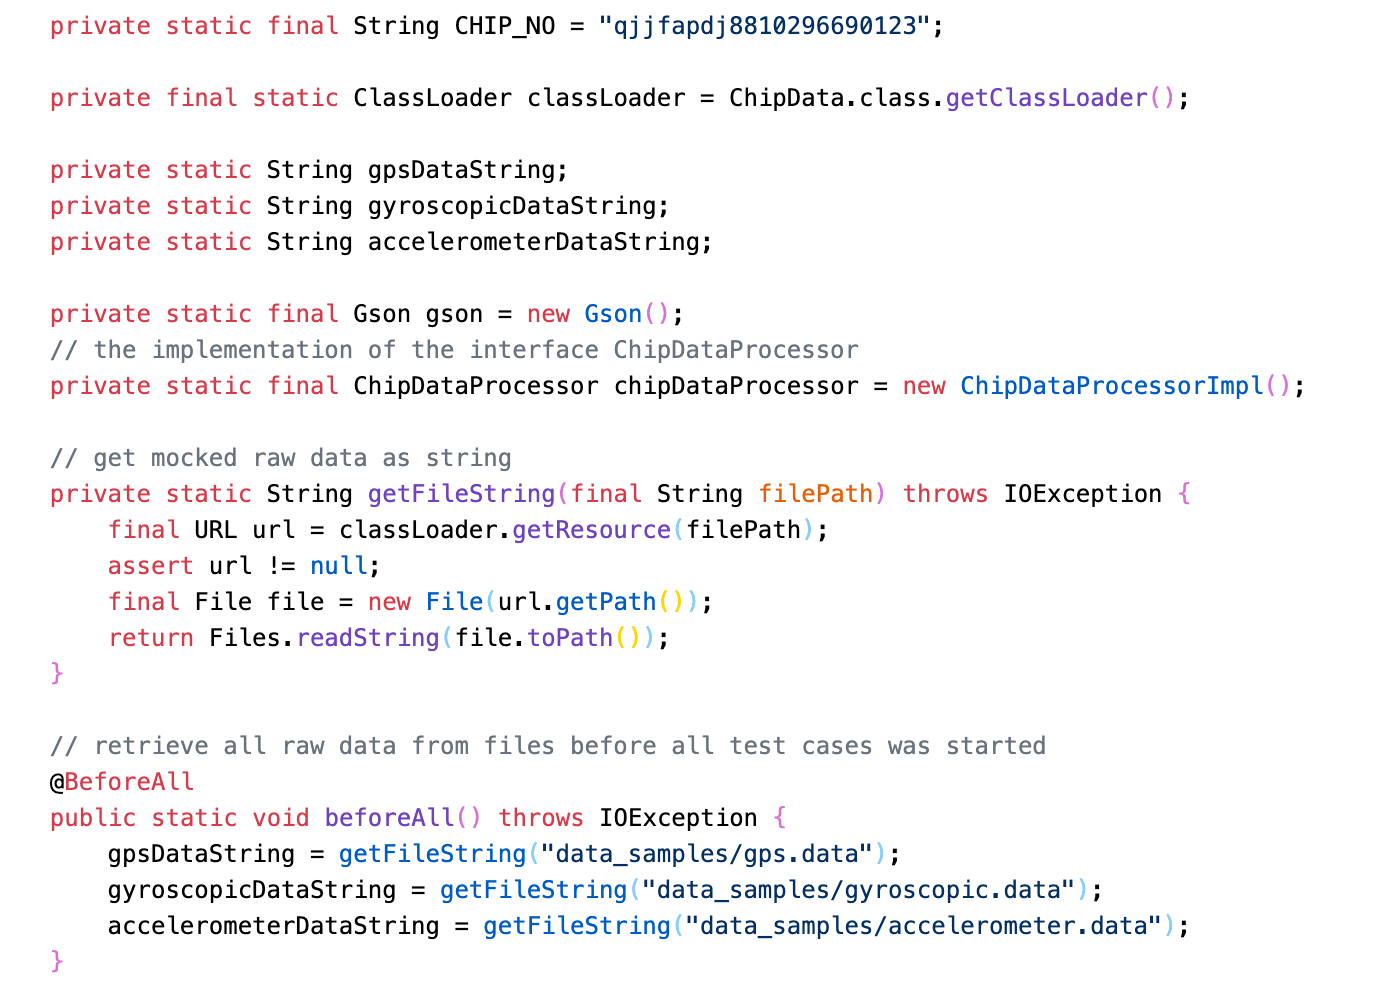
\includegraphics[width=4.4in, valign=m]{./img/f14-t1-testcase-2-preparation.png}
		\label{fig:t1-preparation}}
	\hfil
	\subfloat[Assertion of the Test Unit]{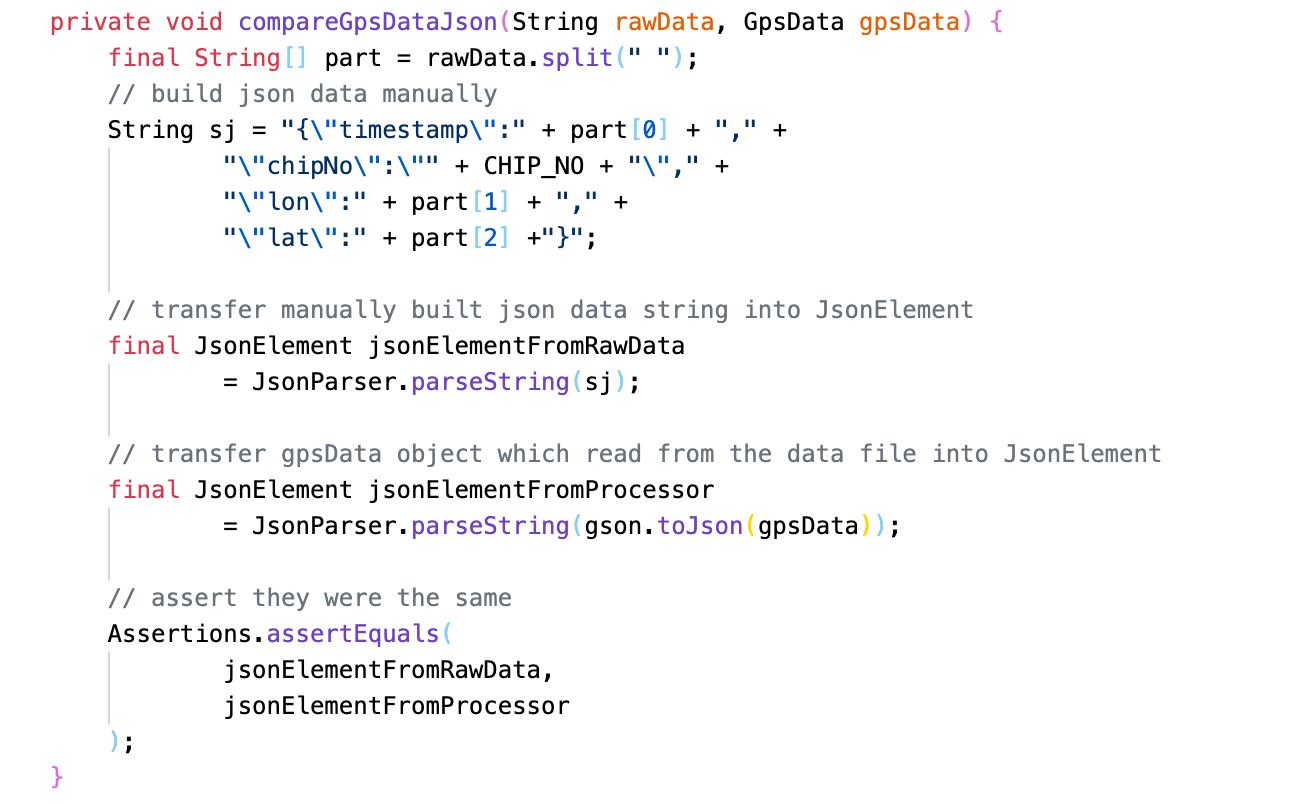
\includegraphics[width=3.8in, valign=m]{./img/f15-t1-testcase-3-equal.png}
		\label{fig:t1-assertion}}
	\subfloat[Test Unit]{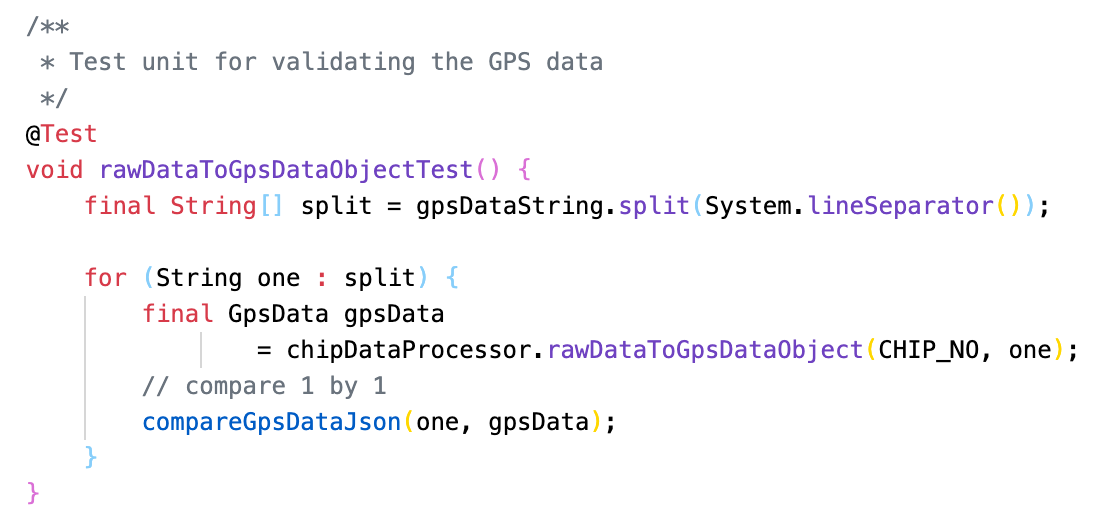
\includegraphics[width=3.2in, valign=m]{./img/f13-t1-testcase-1-test-unit.png}
		\label{fig:t1-test-unit}}
	\caption{Test Case Code of Task 1}
	\label{fig:test-code-t1}
\end{figure}

\begin{figure}[!htp]
	\centering
	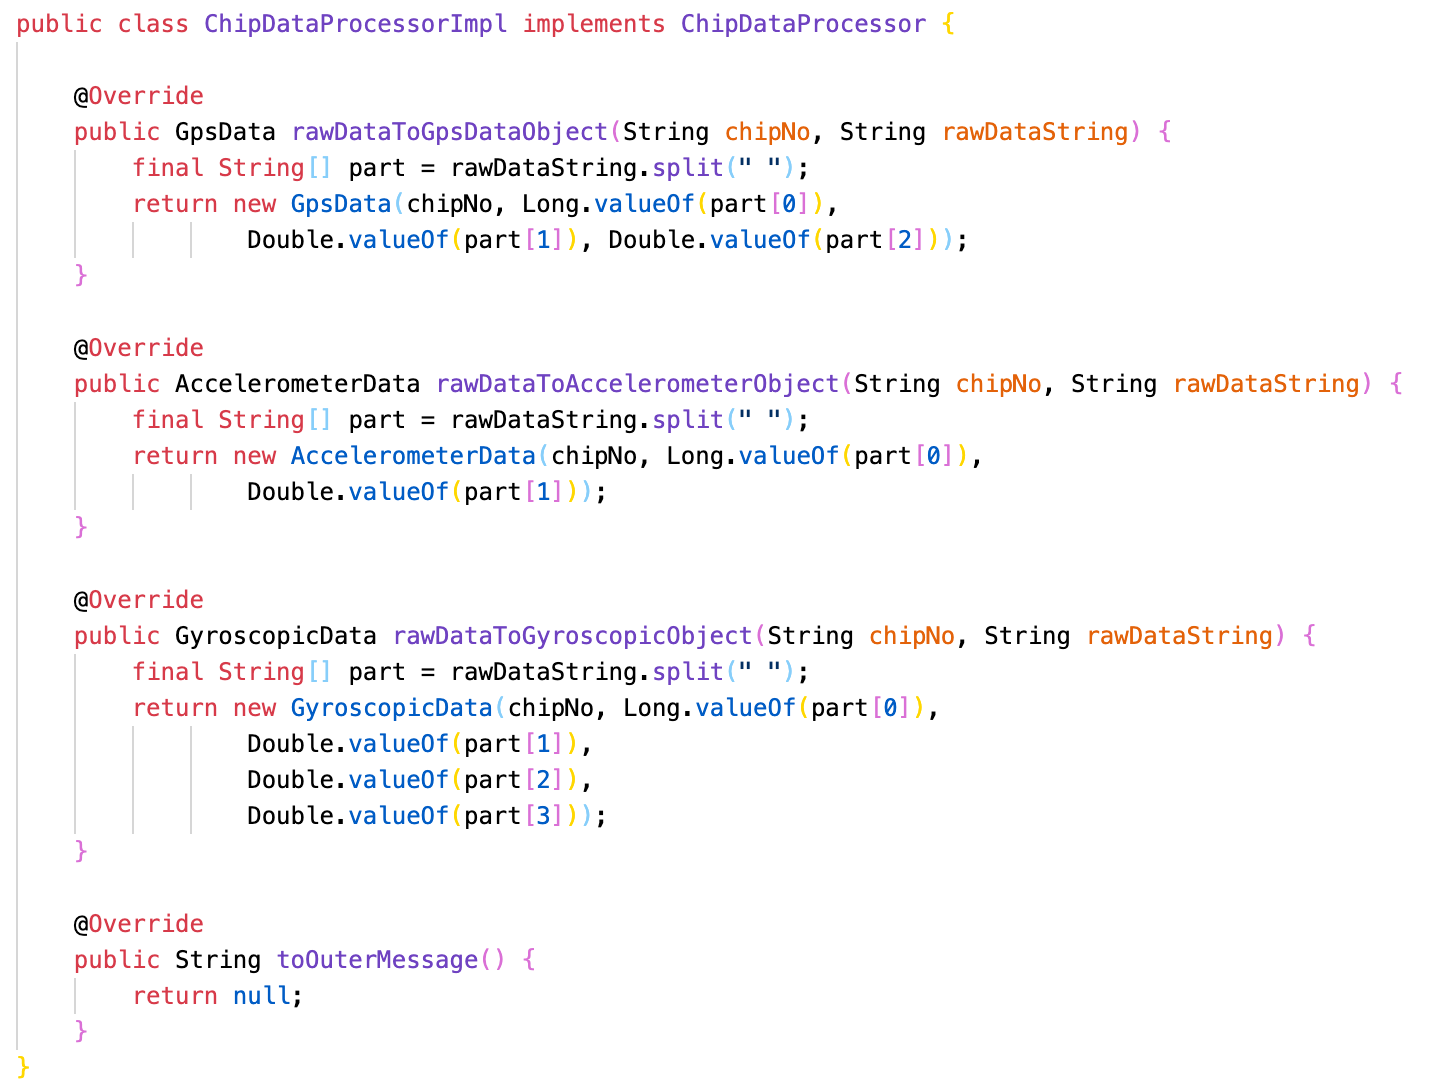
\includegraphics[width=0.7\textwidth]{./img/f18-intf-impl.png}
	\caption{Implementation of the Interface \textit{ChipDataProcessor}}
	\label{fig:intf-impl}
\end{figure}

\begin{figure}[!htp]
	\centering
	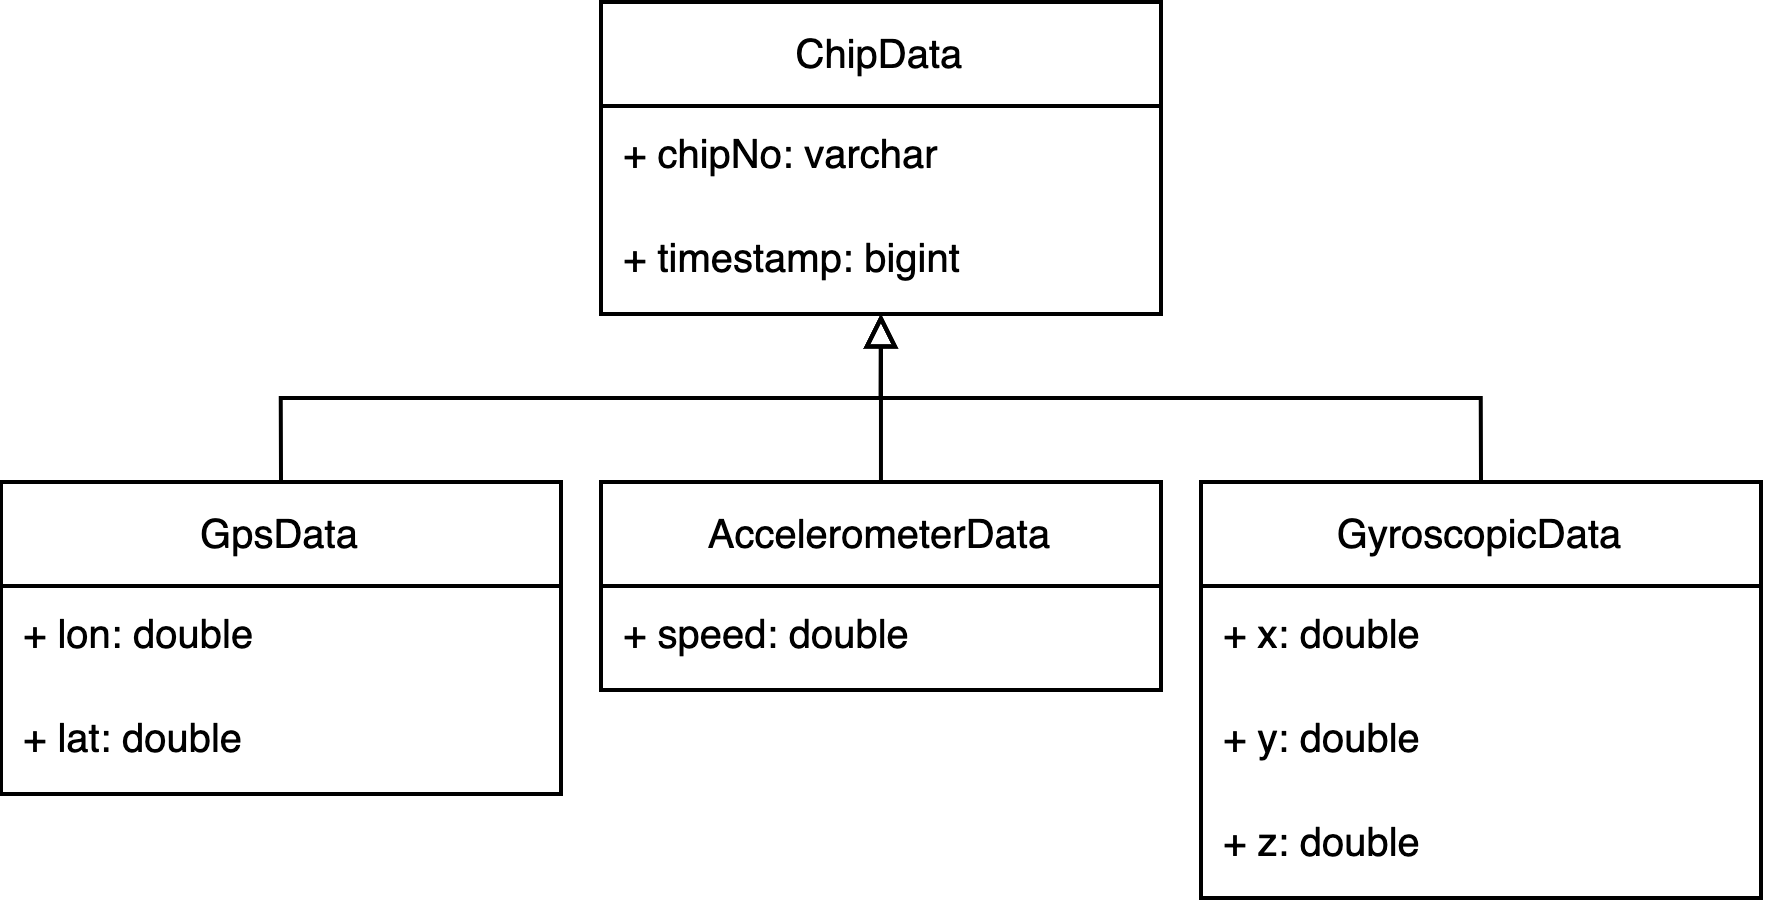
\includegraphics[width=0.6\textwidth]{./img/f17-class-diagram.png}
	\caption{Class Diagram of the Data Objects}
	\label{fig:class-diagram}
\end{figure}

\end{document}
\endinput